\documentclass{beamer}

\mode<presentation>
{
  \usetheme{Madrid}      % or try Darmstadt, Madrid, Warsaw, ...
  \usecolortheme{default} % or try albatross, beaver, crane, ...
  \usefonttheme{professionalfonts}  % or try serif, structurebold, ...
  \setbeamertemplate{navigation symbols}{}
  \setbeamertemplate{caption}[numbered]
} 

\usepackage{physics}
\usepackage[english]{babel}
% \usepackage[utf8]{inputenc}
\usepackage[T1]{fontenc}
\usepackage{xcolor}
\newcommand{\iu}{{i\mkern1mu}}


\title[Wobbling Motion]{DESCRIPTION OF THE WOBBLING MOTION THROUGH A BOSON METHOD}
\author{Robert Poenaru}
\institute{DFT, IFIN-HH}
\date{\today}

\begin{document}

\begin{frame}
  \titlepage
  \vspace{1em} Doctoral School of Physics, UB\\
  \vspace{1em}\emph{Scientific Coordinator}: A. A. Raduta
\end{frame}

\begin{frame}{Outline}
\tableofcontents
\end{frame}

\section{Nuclear shapes}

\begin{frame}
  \frametitle{Nuclear Deformation}

  \begin{exampleblock}{Nuclear Radius}
    The \textbf{shape} of the nucleus is most generally described in terms of the \emph{nuclear radius}:
    \begin{align}
      R(\theta,\varphi;t)=R_0\left(1+\sum_{\lambda=0}^{^\infty}\sum_{\mu=-\lambda}^\lambda\alpha_{\lambda\mu}(t)Y_\lambda^\mu(\theta,\varphi)\right)
    \end{align}
  \end{exampleblock}
\begin{itemize}
  \item The $\alpha_{\lambda\mu}$ are collective coordinates $\Longrightarrow$ \emph{vibrations of the nucleus}.
  \item $Y_\lambda^\mu$ are the spherical harmonics.
\end{itemize}
\end{frame}


\begin{frame}{Nuclear shapes}
  Most nuclei are spherical or axially symmetric in the ground state.
    \begin{figure}
      \centering
      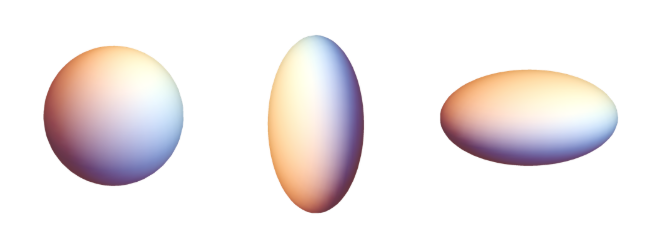
\includegraphics[scale=0.4]{figures/nuclear_shapes.png}
      \caption{\textbf{Spherical:} $\beta_2=0$ ; \textbf{Prolate:} $\beta_2>0$ ; \textbf{Oblate:} $\beta_2<0$}
    \end{figure}
  \end{frame}

\begin{frame}
  \frametitle{Quadrupole deformations}
  \begin{itemize}
    \item Most relevant vibrational degrees of freedom in nuclei.
    \item Play a crucial role in the rotational spectra of nuclei.
  \end{itemize}
\begin{block}{Quadrupole radius}
  For pure quadrupole deformations:
  \begin{align}
    R(\theta,\varphi)=R_0\left(1+\sum_\mu\alpha_{2\mu}Y_2^\mu(\theta,\varphi)\right)\ ,
  \end{align}
  Using A. Bohr's description, the coordinates $\alpha_{2\mu}$ can be reduced to only two \emph{deformation parameters}: $\beta_2$ (\emph{eccentricity}) and $\gamma$ (\textbf{triaxiality}).
\end{block}
\end{frame}

\section{Triaxial Shapes}

\begin{frame}
  \frametitle{Nuclear triaxiality}
\begin{itemize}
  \item Besides the axially symmetric shapes (i.e., spherical, prolate, and oblate), nuclei can be \textbf{triaxial} $\Longrightarrow$ lack of symmetry along any of the principal axes.
  \item The asymmetry is given by the non-zero value of $\gamma$.
\end{itemize}
\begin{figure}
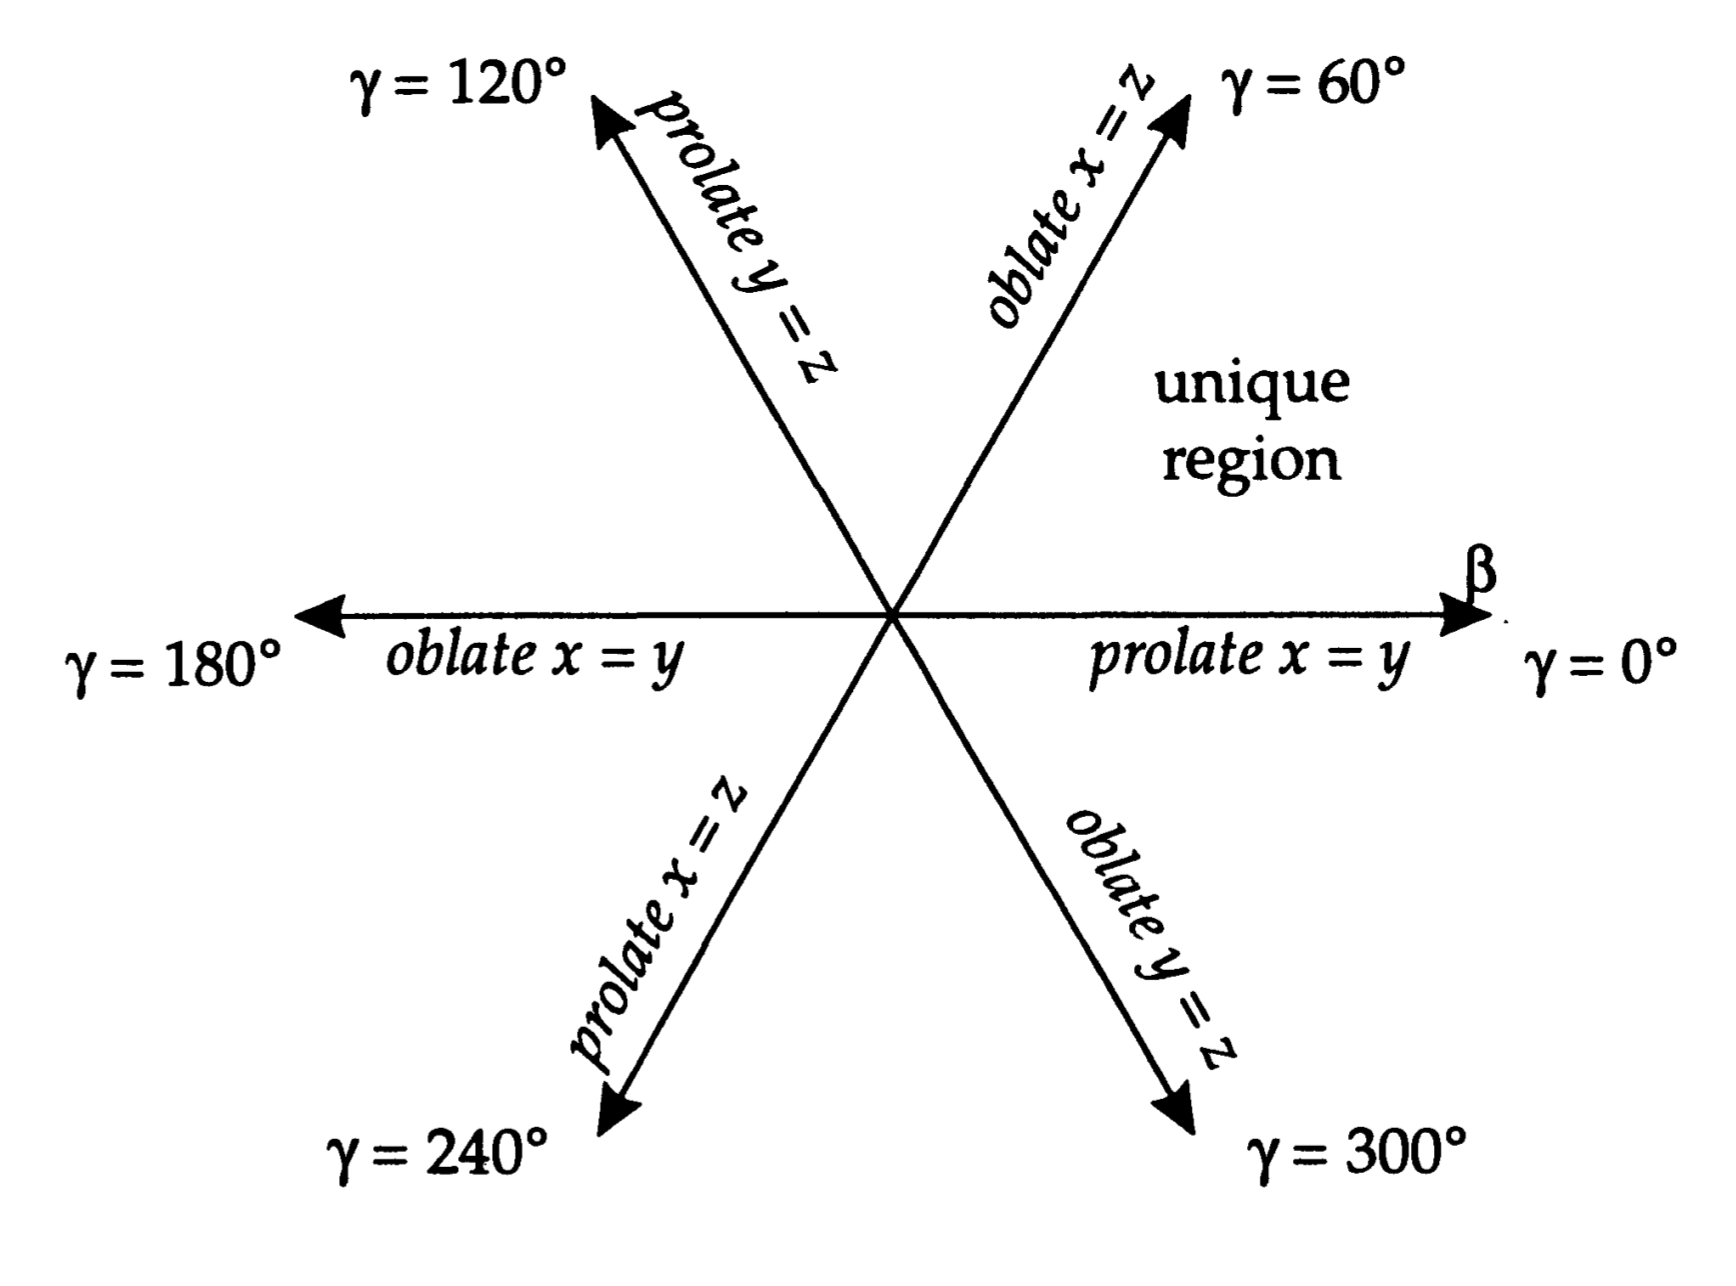
\includegraphics[scale=0.25]{figures/beta-gamma-plane.png}  
\end{figure}
\end{frame}

\begin{frame}
  \frametitle{Triaxial ellpsoid}
  Schematic example with a triaxial ellipsoid ($\gamma\neq0$)  $\beta_2>0$.
  \begin{figure}
    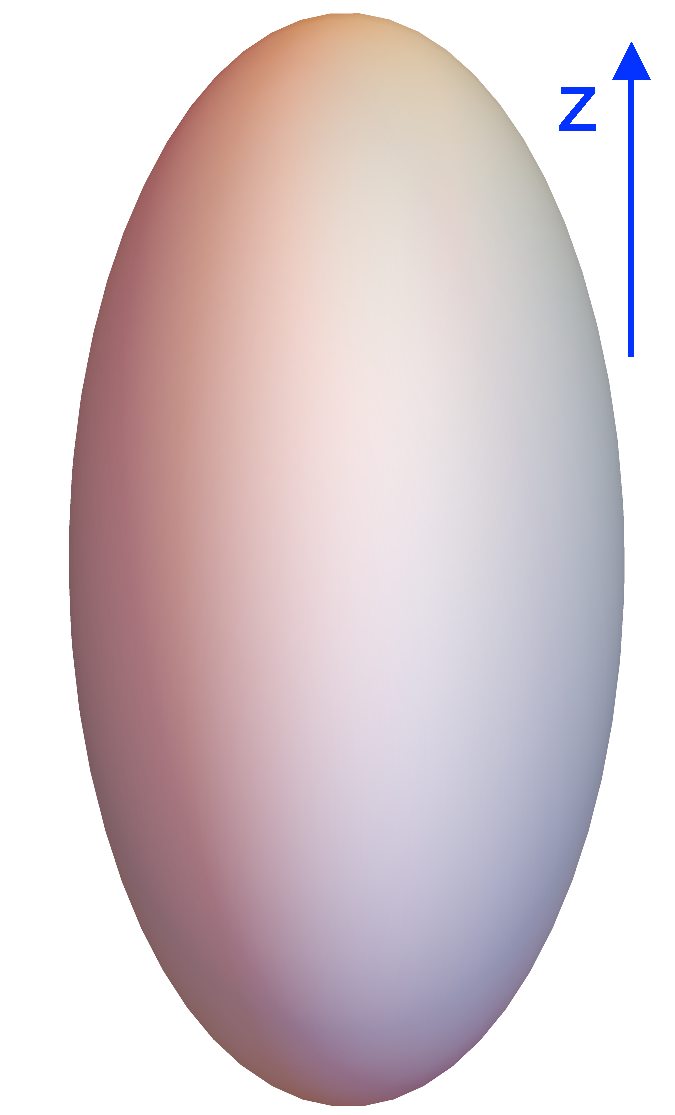
\includegraphics[scale=0.25]{figures/ellipsoid-side-view-2.pdf}
    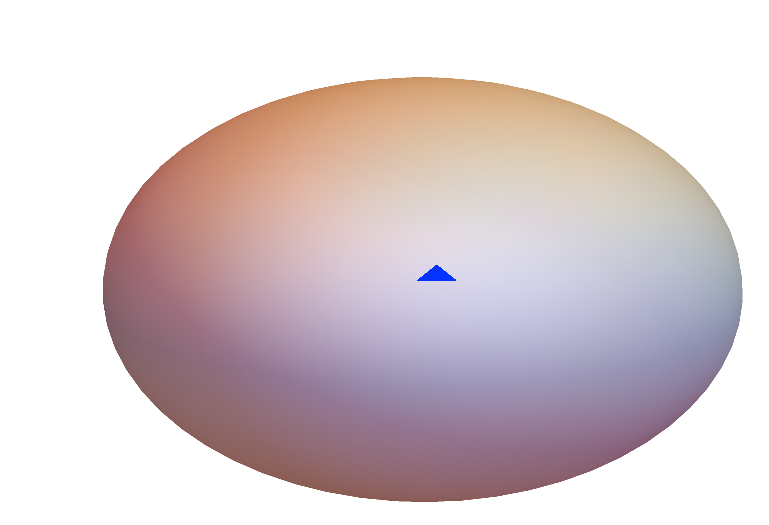
\includegraphics[scale=0.3]{figures/ellipsoid-top-view.pdf}
    \caption{\textbf{Left:} side-view. \textbf{Right:} top view.}
  \end{figure}
\end{frame}

\begin{frame}
  \frametitle{Nuclear triaxiality}

\begin{itemize}
  \item Probing triaxiality experimentally is a real challenge (e.g., large and complex detector setups).
  \item Only two fingerprints known so far: \textbf{chiral motion} (Frauendorf, 1997) and \textbf{wobbling motion} (Bohr and Mottelson, 1975).
\end{itemize}

\begin{block}{Wobbling Motion (WM)}
  \begin{itemize}
    \item Collective effect $\rightarrow$ \emph{unique} to triaxial nuclei.
    \item Predicted almost 50 years ago, first experimental confirmation: in 2001 (Odegard et al.) for $^{163}$Lu.
    \item In present, few wobblers are experimentally confirmed in the mass regions: $A\approx130,160,180$ $\rightarrow$ {\color{brown}A list of all known wobblers will be available in my PhD thesis (Chapter 3)}. 
  \end{itemize}
\end{block}

\end{frame}

\section{Wobbling motion}

\begin{frame}{Wobbling motion}
  \begin{columns}
    \begin{column}{0.47\textwidth}
    \begin{block}{Triaxial nuclei}
        A triaxial nucleus can rotate about any of the three axes.

        \vspace{0.3cm}
        The rotational angular momentum (a.m.) is NOT aligned along any of the body-fixed axes $\Longrightarrow$ \textbf{precesses} and \textbf{wobbles} around the axes with the largest MOI. 
    \end{block}
    \end{column}
    \begin{column}{0.53\textwidth}
        \begin{figure}
          \centering
          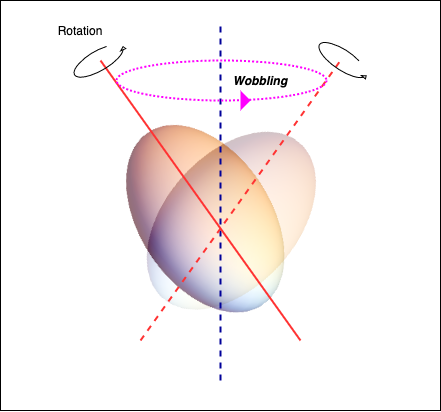
\includegraphics[scale=0.35]{figures/wobbling_drawing.png}
          \caption{Schematic representation for the nuclear wobbling motion.}
          \label{wobbling_picture}
      \end{figure}
  
    \end{column}
    \end{columns}
\end{frame}

\begin{frame}
  \frametitle{Wobbling Bands}
  
  \begin{columns} 
  \column{.5\textwidth} 
  \begin{block}{Wobbling bands}
    Sequences of $\Delta I=2\hbar$ rotational bands that are built on different \textit{wobbling phonon excitations} ($n_w=0,1,\dots$).

    Oscillatory behavior, with a \emph{tilting angle} for the angular momentum proportional to $n_w$ $\longrightarrow$ \textbf{harmonic-like motion}.
  \end{block}
  
  \column{.5\textwidth}
  \begin{figure}
      \centering
      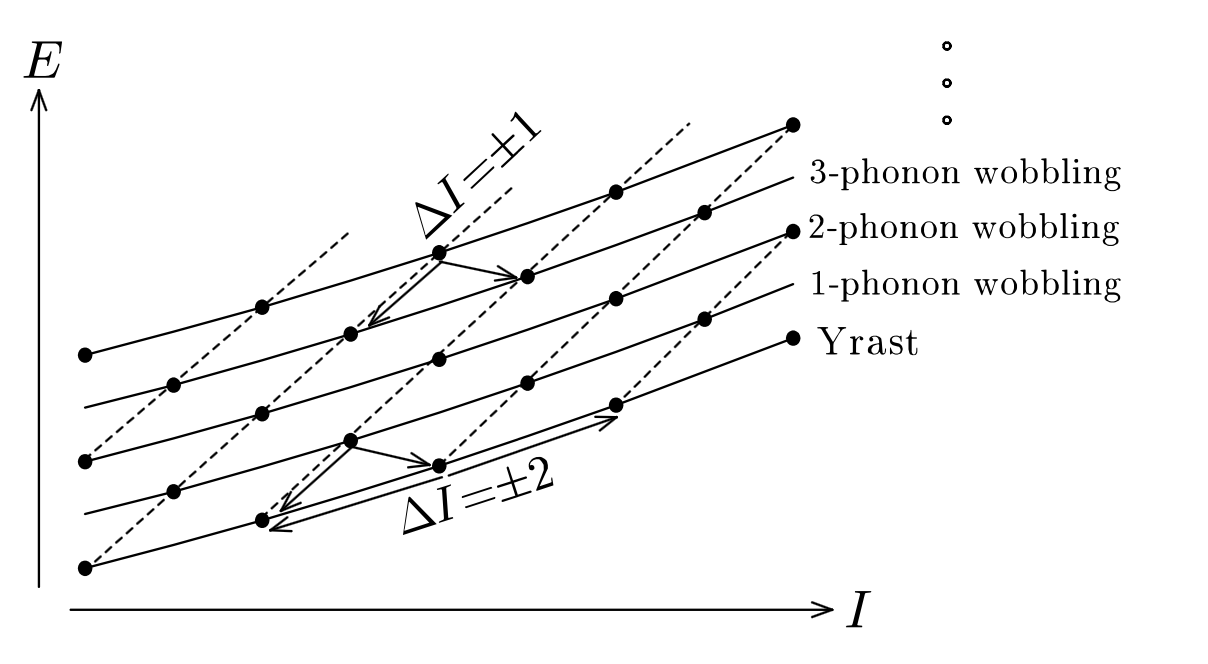
\includegraphics[scale=0.14]{figures/wobblingBands.png}
      \caption{Rotational-band structures of the wobbling motion.}
    \end{figure}
  \end{columns}
    \begin{itemize}
      \item For $^{163}$Lu: $n_w=0,1,2,3$ wobbling phonon numbers, respectively.
      \item Nuclei have \textbf{large} quadrupole moments
      \item \textbf{Strong E2} character for the electro-magnetic transitions.
    \end{itemize}

\end{frame}

\begin{frame}
  \frametitle{Even-Even vs. Even-Odd Nuclei}
\begin{block}{Theoretical frameworks for \textbf{even-mass} nuclei}
  \begin{enumerate}
    \item \emph{Harmonic Approximation(s)} (Bohr and Mottelson, 1975)
    \item Triaxial-Rotor-Model (Davydov and Filippov, 1958)
    \item Boson-approximations (Tanabe, 1971)
  \end{enumerate}
\end{block}

\begin{block}{Theoretical frameworks for \textbf{odd-mass} nuclei}
  \begin{enumerate}
    \item Particle Rotor Model (Hamamoto, 2002)
    \item Tilted-axis wobbling (Frauendorf and Meng, 1997)
    \item RPA, Mean-Field Theories, GCM+AMP...
    % \item Tilted-Axis wobbling (R. Budaca, 2018)
  \end{enumerate}
\end{block}

\begin{exampleblock}{Recent work on wobbling motion}
  \begin{itemize}
    \item RPA for $^{163}$Lu, Raduta et al (PRC, 2017)
    \item Tilted-axis wobbling for $^{135}$Pr, R. Budaca (PRC, 2018)
    \item PRM for $^{163}$Lu, R. Poenaru (IJMPE, 2021)
  \end{itemize}
\end{exampleblock}

\end{frame}

\section{Theoretical formalism}

% \subsection{Hamiltonian}

\begin{frame}
  Based on the work: \textbf{AA Raduta, CM Raduta, R Poenaru, Journal of Physics G: Nuclear and Particle Physics 48 (1), 015106, 2020}
  \frametitle{Theoretical formalism - Even-Odd Nuclei}
  \begin{exampleblock}{Description of WM for an even-odd nucleus}
    \begin{itemize}
      \item one single-particle (nucleon) \emph{coupled} to an \emph{even-even} triaxial core.
      \item the nucleon is moving in a quadrupole deformed mean-field generated by the core
      \item particle + rotor coupling drives the entire system to large (and stable) deformations ($\epsilon\sim0.2-0.4$).
    \end{itemize}
  \end{exampleblock}
Hamiltonian:
\begin{align}
  \hat{H}_\text{rot}=\sum_{k=1}^3A_k\left(\hat{I}_k-\hat{j}_k\right)^2\ .
\end{align}
$A_k\rightarrow$ inertia parameters: $A_k=(2\mathcal{I}_k)^{-1}$.
\end{frame}

\begin{frame}
  \frametitle{Theoretical Formalism - Rotational Hamiltonian}

  Expanding $\hat{I}_2$ up to first order (particle is \emph{rigidly coupled} to the core):
  \begin{align}
    \hat{I}_2=I\left(1-\frac{1}{2}\frac{\hat{I}_1^2+\hat{I}_3^2}{I^2}\right)\ ,
  \end{align}
can help re-write the initial Hamiltonian: % $I$ is the \textbf{total angular momentum of the nucleus}.
\begin{exampleblock}{Rigid coupling Hamiltonian: $\mathbf{j}=(j\cos\theta,j\sin\theta,0)$}
  \begin{align}
    \hat{H}_\text{rot}&={\color{red}AH'}+{\color{blue}H_{sp}}+{\color{magenta}\text{s.t.}}\ ,\\
    {\color{red}H'}&=\hat{I}_2^2+u\hat{I}_3^2+2v_0\hat{I}_1\ ,\ {\color{blue}H_{sp}}=\sum_{k=1}^2A_k\hat{j}_k^2\ ,\ {\color{magenta}\text{s.t.}}=A_1I^2-A_2j_2I\ ,\\
    1>u&=\frac{A_3-A_1}{A}>-1\ ,\ v_0-\frac{A_1j_1}{A}\ ,\ A=A_2\left(1-\frac{j_2}{I}\right)>0
  \end{align}
\end{exampleblock}
\end{frame}

\begin{frame}
  \frametitle{Rotational Hamiltonian}
  \begin{itemize}
    \item $H'$ looks like the Hamiltonian for a triaxial rigid rotator + constrained (cranked) to move along the $1$-axis.
    \item The a.m. algebra is defined as:
    \begin{align}
      \hat{I}_\pm=\hat{I}_2\pm \iu\hat{I}_3\ &,\ \hat{I}_0=\hat{I}_1\ ,\\
      \left[\hat{I}_-,\hat{I}_+\right]=2\hat{I}_0\ &,\ \left[\hat{I}_\mp,\hat{I}_0\right]=\mp\hat{I}_\mp\ .
    \end{align}
  \end{itemize}
\begin{block}{Hamiltonian + Schrodinger Equation}
  \begin{align}
    H'=a\left(\hat{I}_+^2+\hat{I}_-^2\right)+b\left(\hat{I}_+\hat{I}_-+\hat{I}_-\hat{I}_+\right)+c\hat{I}_0\ ,
  \end{align}
  \begin{align}    
    H'\ket{\Psi}=E\ket{\Psi}\ .
  \end{align}
\end{block}
\end{frame}

% \subsection{Angular momentum}

\begin{frame}
  \frametitle{Angular Momentum Representation}
  The a.m. ladder operators are re-defined in terms of new variables ${\color{brown}q},{\color{blue}d/dq}$:
  \begin{align}
    \hat{I}_\mp=\iu\frac{{\color{brown}c}\pm {\color{brown}d}}{\color{brown}s}\left(I\mp\hat{I}_0\right)\ ,\ \hat{I}_0=I{\color{brown}cd}-{\color{brown}s}{\color{blue}\frac{d}{dq}}\ .
  \end{align}
  \begin{columns} 
    \column{.5\textwidth}
    $s,c,d$ are the \textbf{Jacobi Elliptic Functions}:
    \begin{align}
      s&=\text{sn}({\color{brown}q},k)\ ,\ c=\text{cn}({\color{brown}q},k)\ \\
      d&=\text{dn}({\color{brown}q},k)\ ,
    \end{align}
    The functions are periodic in $q$, with the periods $4K$ ($s$), $4K$ ($c$), and $2K$ ($d$).
    \column{.5\textwidth}
    \begin{figure}
      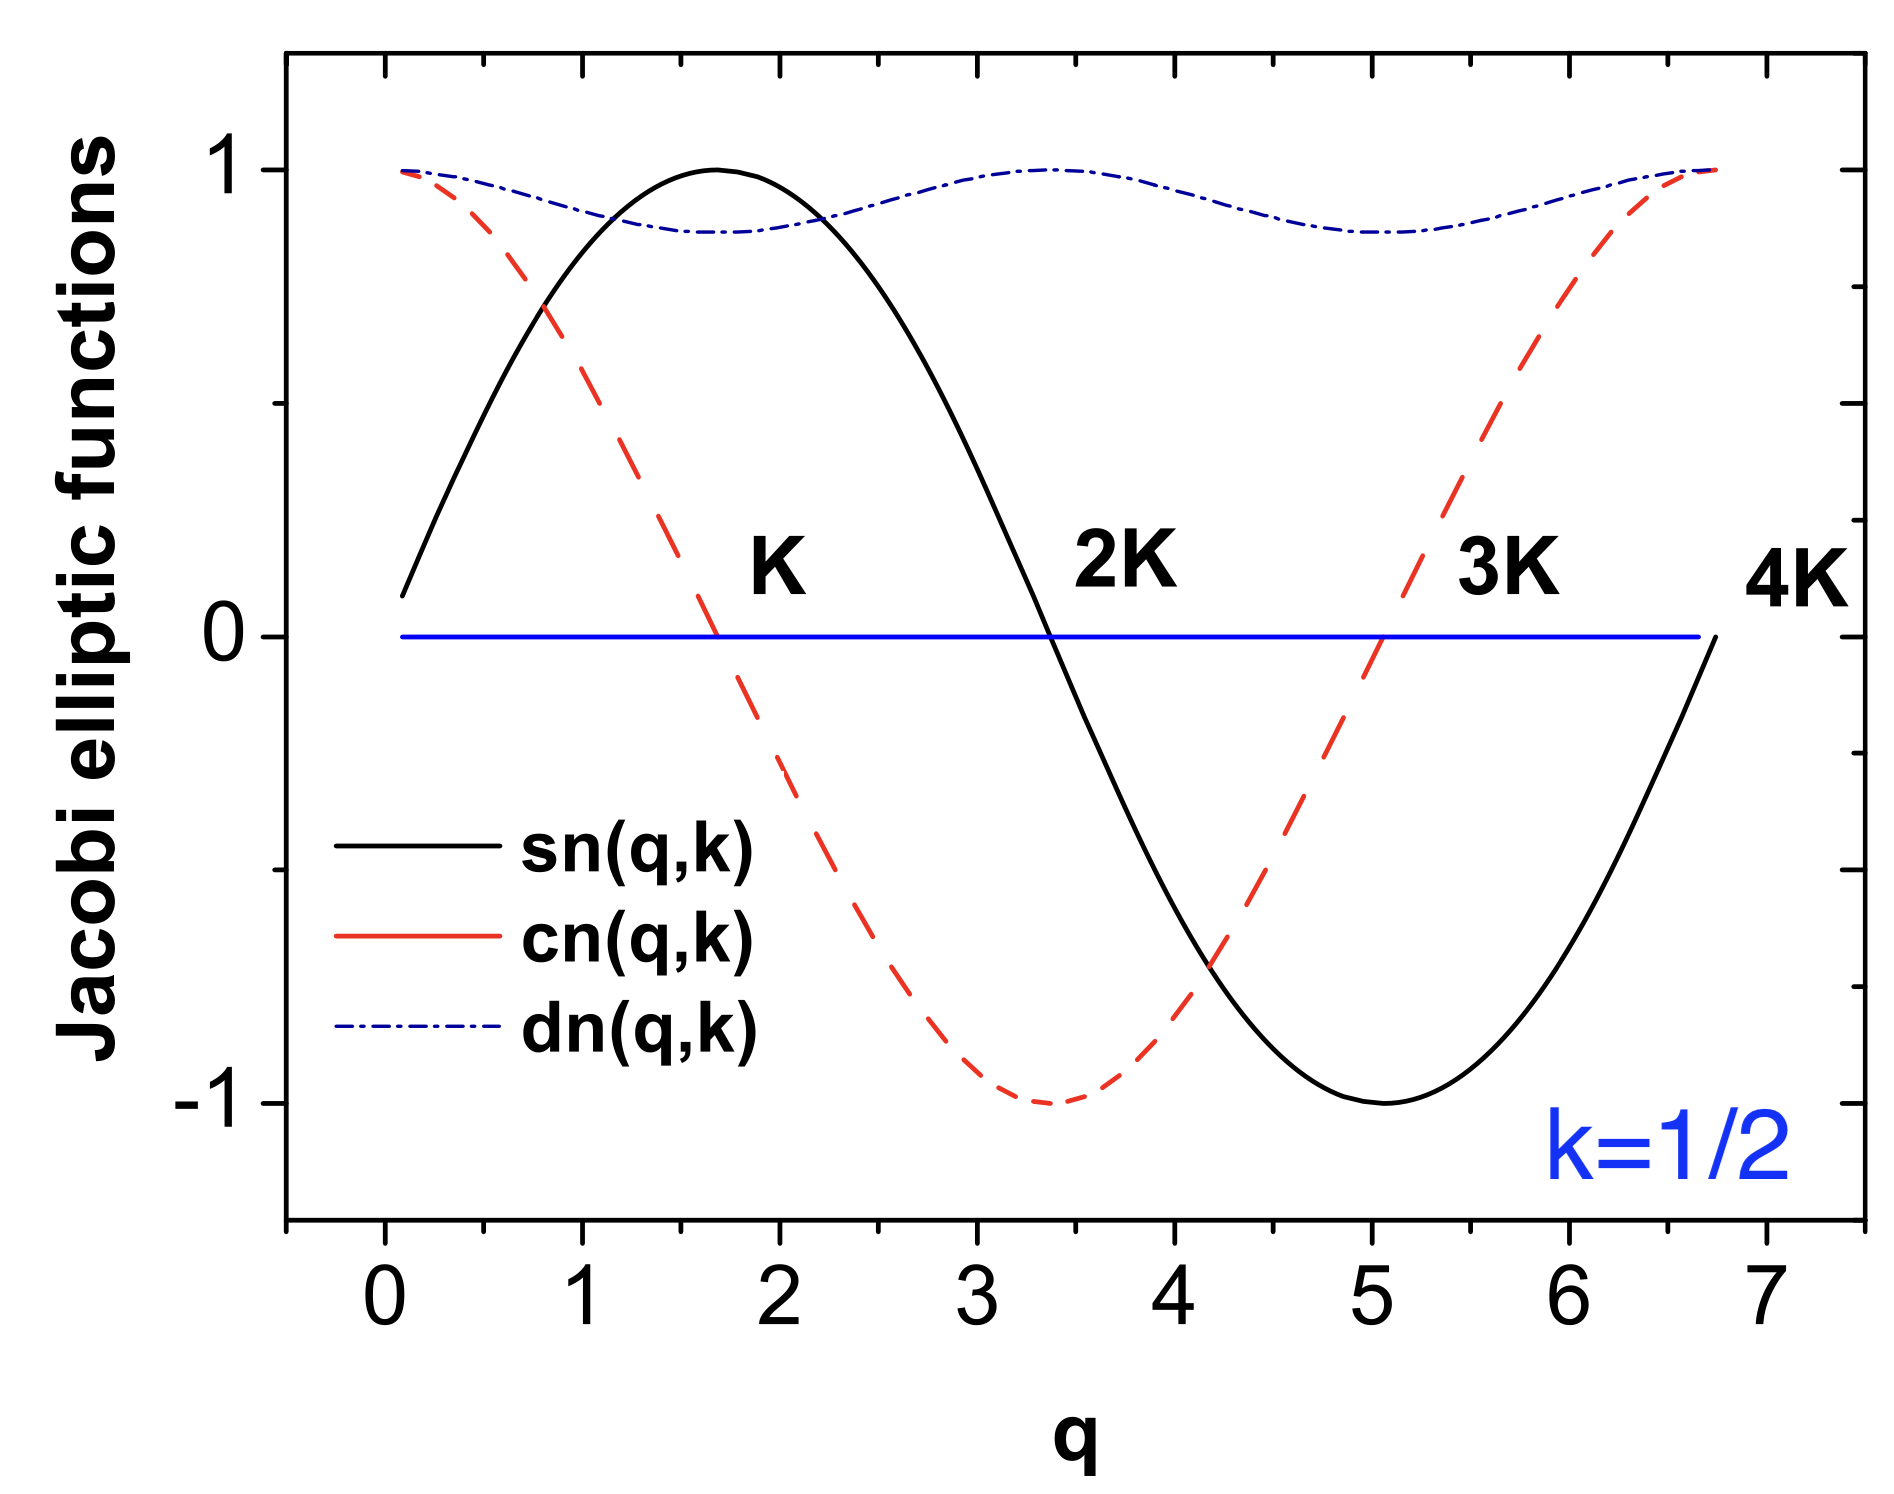
\includegraphics[scale=0.18]{figures/jacobi-functions.png}
    \end{figure}
    \end{columns}
\end{frame}

\begin{frame}
  \frametitle{Coordinate representation}
  The variable $q$ is defined in terms of $k$ ($0<k^2<1$):
\begin{align}
  q&=\int_0^\varphi\left(1-k^2\sin^2(t)\right)^{-1/2}dt=F(\varphi,k)\ ,\ \varphi=F^{-1}(q,k)\ ,\\
  s&=\sin\varphi\ ,\ c=\cos\varphi\ ,\ d=\sqrt{1-k^2s^2}\ ,\ k=\sqrt{|u|}\ .
\end{align}
\begin{exampleblock}{New Hamiltonian}
  \begin{align}
      H'=-\frac{d^2}{dq^2}-2v_0s\frac{d}{dq}+I(I+1)s^2k^2+2v_0cdI\ ,
  \end{align}
  with the associated \emph{Schrodinger Equation} (fully separated Kinetic and Potential terms):
  \begin{align}
    \left[\frac{d^2}{dq^2}+V(q)\right]\Psi=E\Psi
  \end{align}
\end{exampleblock}
\end{frame}

\begin{frame}
  \frametitle{The "Elliptic" Potential}
\begin{block}{The expression of $V(q)$}
  With the elliptic functions $s,c,d$, and arbitrary $k$:
  \begin{align}
    V(q)&=\left[I(I+1)k^2+v_0^2\right]s^2+(2I+1)v_0cd=V(-q)\ .
  \end{align}
\end{block}
\begin{figure}
  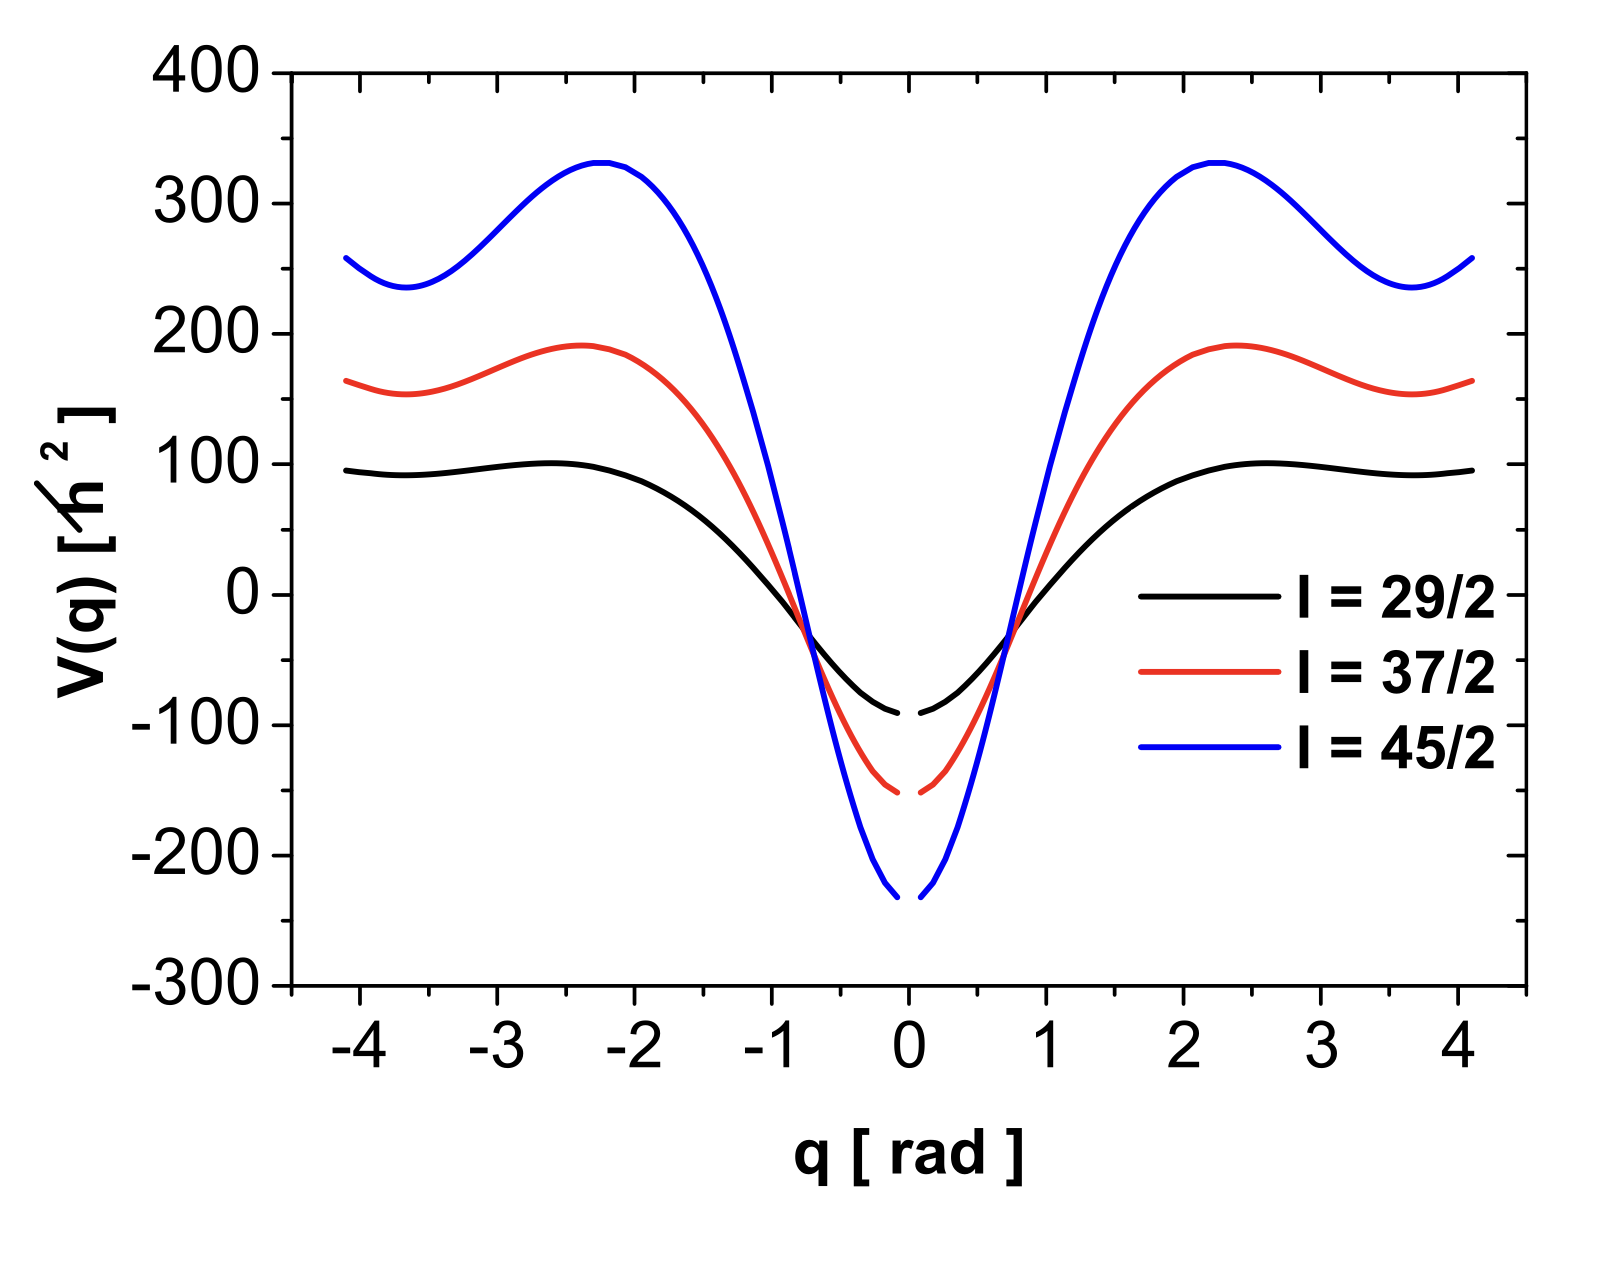
\includegraphics[width=0.48\textwidth]{figures/potential-1.png}
  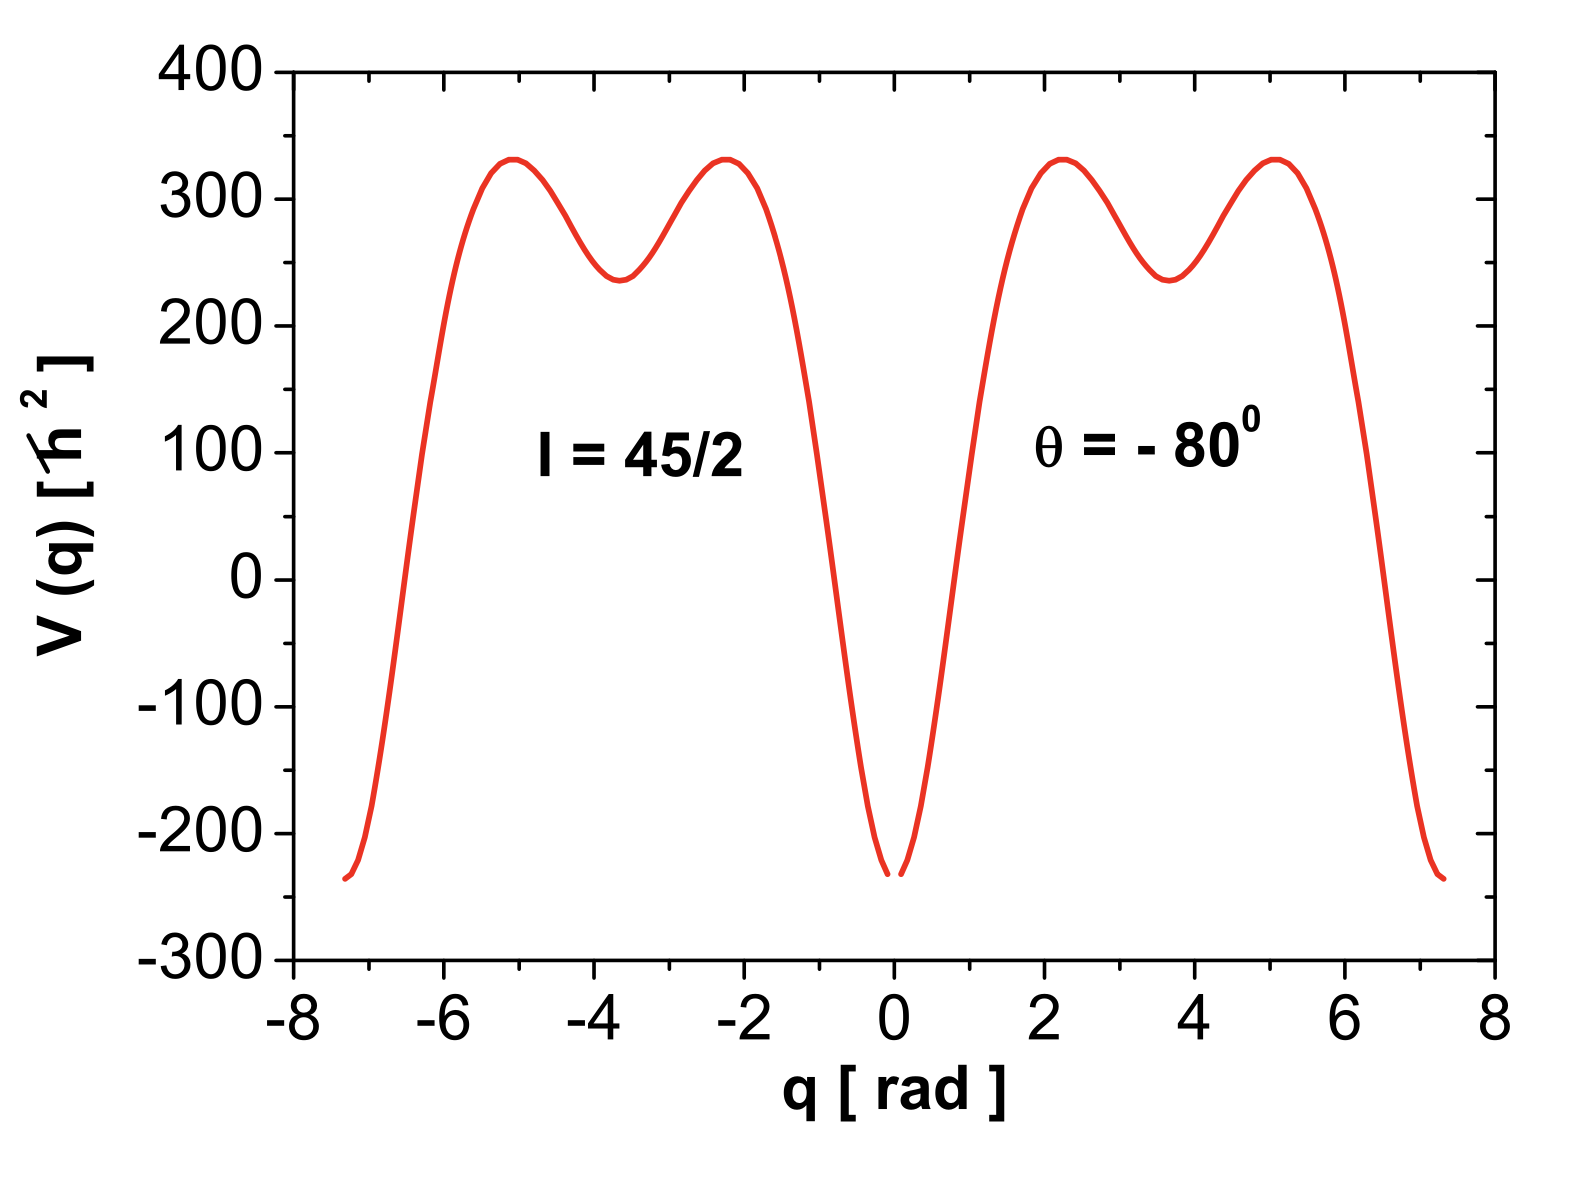
\includegraphics[width=0.48\textwidth]{figures/potential-2.png}
  % 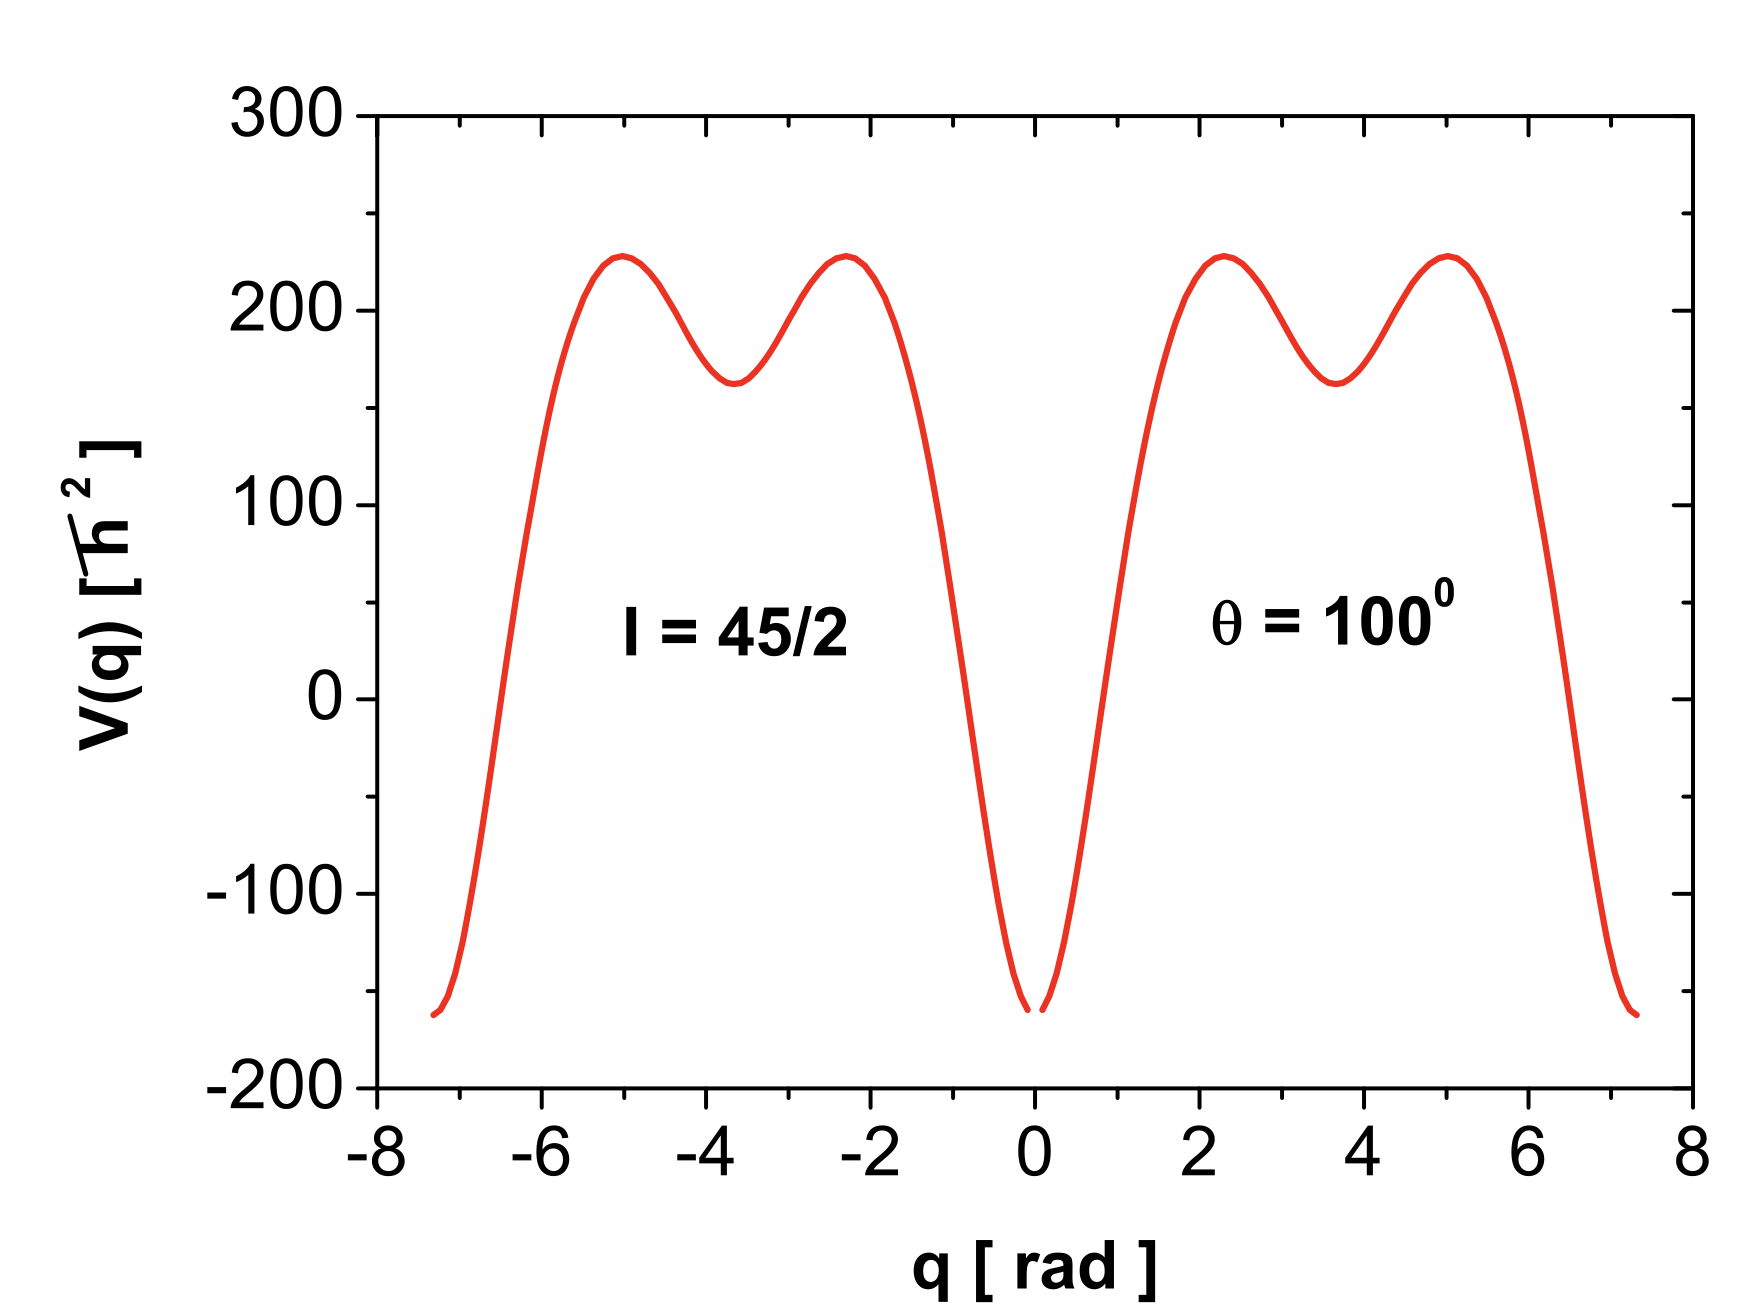
\includegraphics[width=0.3\textwidth]{figures/potential-3.png}
\end{figure}
Local minima states: meta-stable. \emph{Deepest well} states: degenerate.

\end{frame}

% \subsection{Elliptic potential}

\begin{frame}
  \frametitle{The "Elliptic" Potential}
  \begin{columns}
    \column{.5\textwidth}
    \begin{figure}
      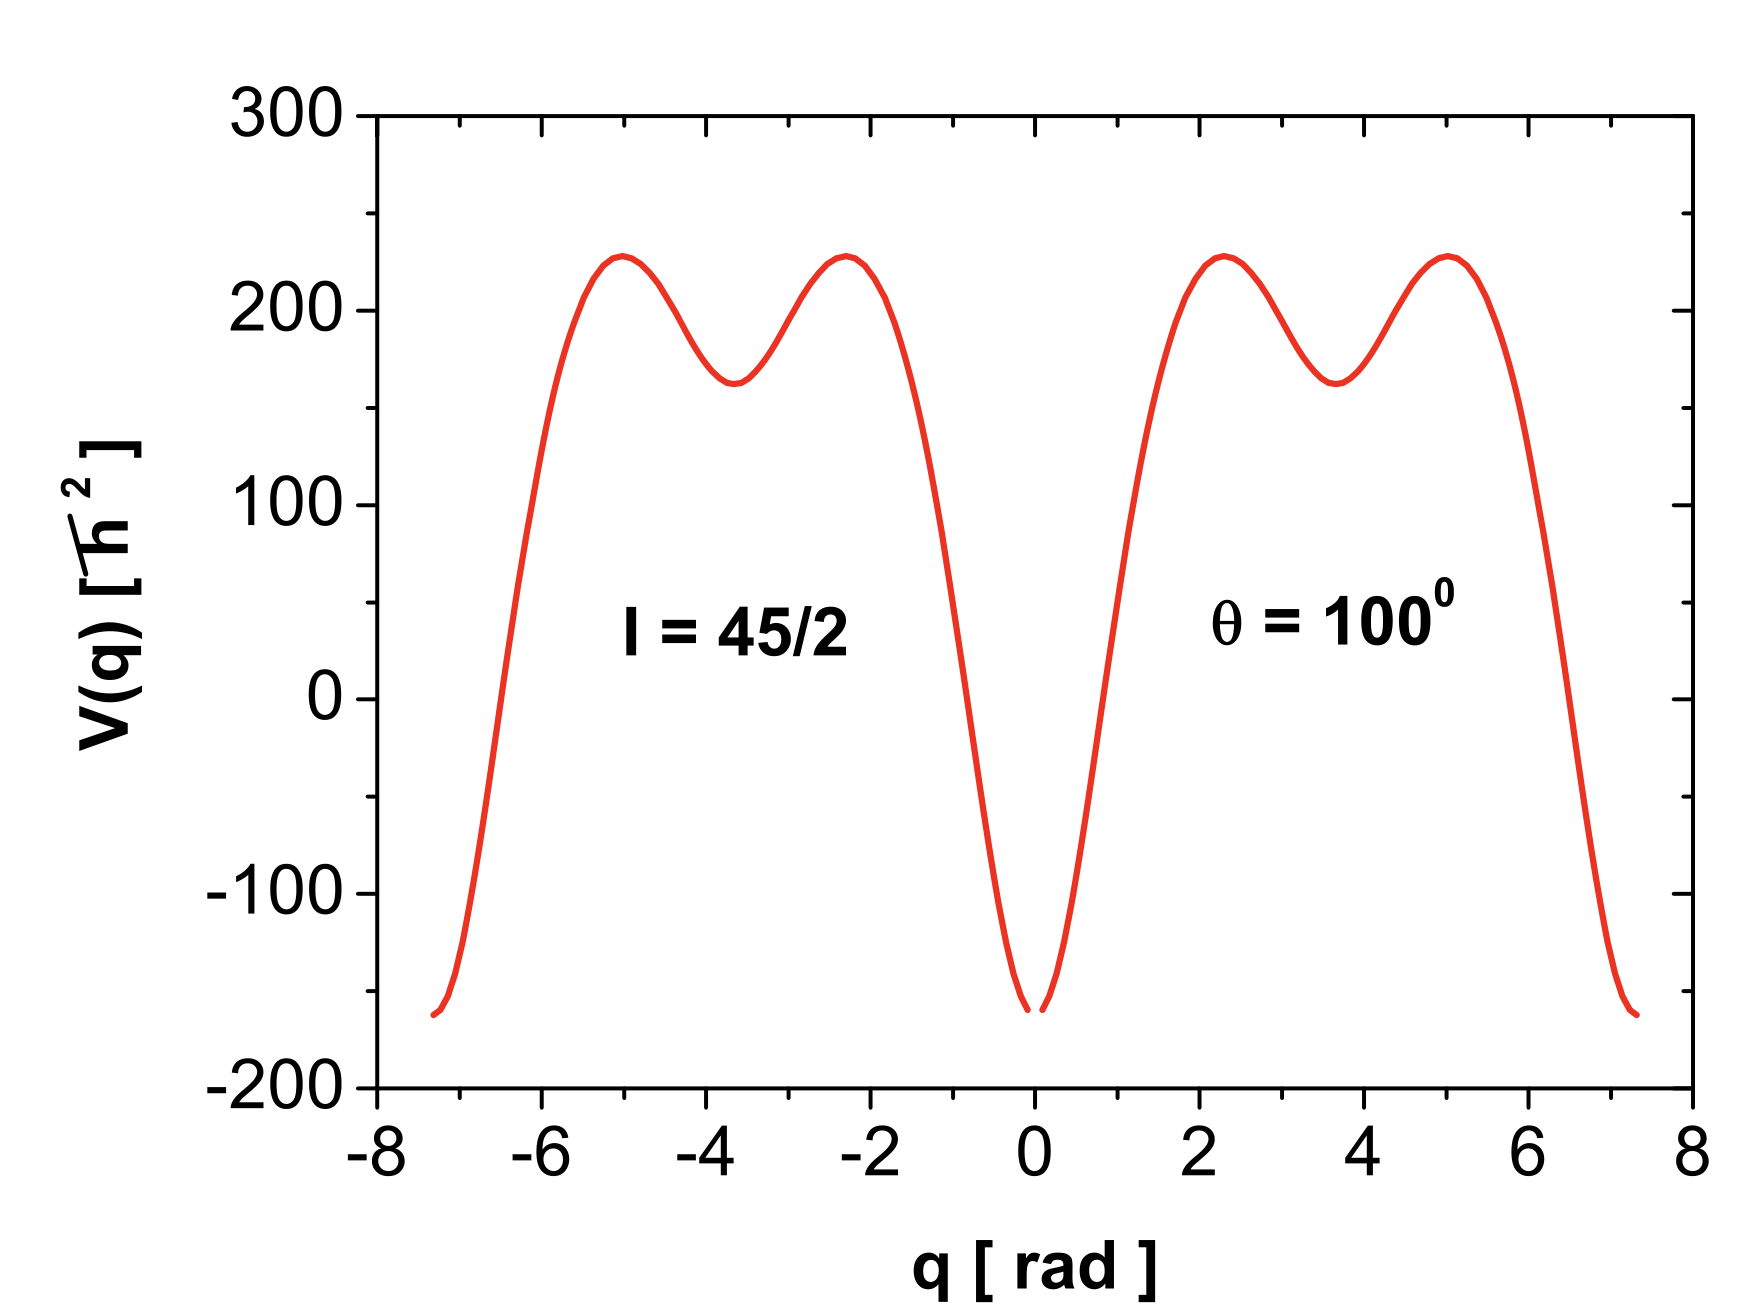
\includegraphics[scale=0.18]{figures/potential-3.png}
    \end{figure}
    \column{.5\textwidth}
    \begin{itemize}
      \item The deepest minima appear at $q=0,\pm4K$.
      \item Meta-stable (local) minima appear at $q=\pm2K$.
    \end{itemize}
  \end{columns}
\end{frame}

% \subsection{Boson description for the a.m.}

\begin{frame}
  \frametitle{Bargmann Mapping - Boson description}
The variables $q$ and $d/dq$ can be mapped to a pair of \textbf{boson operators} ($b,b^\dagger$) via the Bargmann representation of the angular momentum:
\begin{align}
  q\rightarrow b^\dagger\ ,\ \frac{d}{dq}\rightarrow b\ .
\end{align}
\begin{block}{New angular momentum operators}
  This mapping leads to \emph{the first boson expansion of the angular momentum components in literature}.
  \begin{align}
    \hat{I}_+&=\iu\frac{cb^\dagger-db^\dagger}{sb^\dagger}\left(I+Icb^\dagger db^\dagger-sb^\dagger b\right)\ ,\\
    \hat{I}_-&=\iu\frac{cb^\dagger+db^\dagger}{sb^\dagger}\left(I-Icb^\dagger db^\dagger+sb^\dagger b\right)\ ,\\
    \hat{I}_0&=Icb^\dagger db^\dagger-sb^\dagger b\ .
  \end{align}
\end{block}
\end{frame}

\begin{frame}
  \frametitle{Wobbling spectrum}
  \begin{exampleblock}{Harmonic oscillator}
    Expanding $V(q)$ around the deepest minima up to second order in $q$, the spectrum of $H_\text{rot}$ is obtained:
    \begin{align}
      E_n=A_1I^2-(2I+1)A_1j_1-IA_2j_2+\sum_{k=1}^2A_kj_k^2+{\color{red}\hbar\omega\left(n+\frac{1}{2}\right)}\ .
    \end{align}
  \end{exampleblock}
  \begin{itemize}
    \item The frequency $\hbar\omega$ is the so-called \emph{wobbling frequency}.
    \begin{align}
      \hbar\omega_I=f(A_1,A_2,A_3;I)  
    \end{align}
    \item $n$ is the wobbling phonon number $n=0,1,\dots$.
  \end{itemize}
\end{frame}

\begin{frame}
  \frametitle{Wobbling spectrum}
  \begin{itemize}
    \item Recall $H_\text{rot}$ contains the $H'$ Hamiltonian.
    \item The $\hbar\omega$ frequency corresponds to $H_\text{rot}$.
    \item Similarly, $\hbar\omega'$ is the frequency for $E_n'$, corresponding to $H'$.
  \end{itemize}
\begin{figure}
  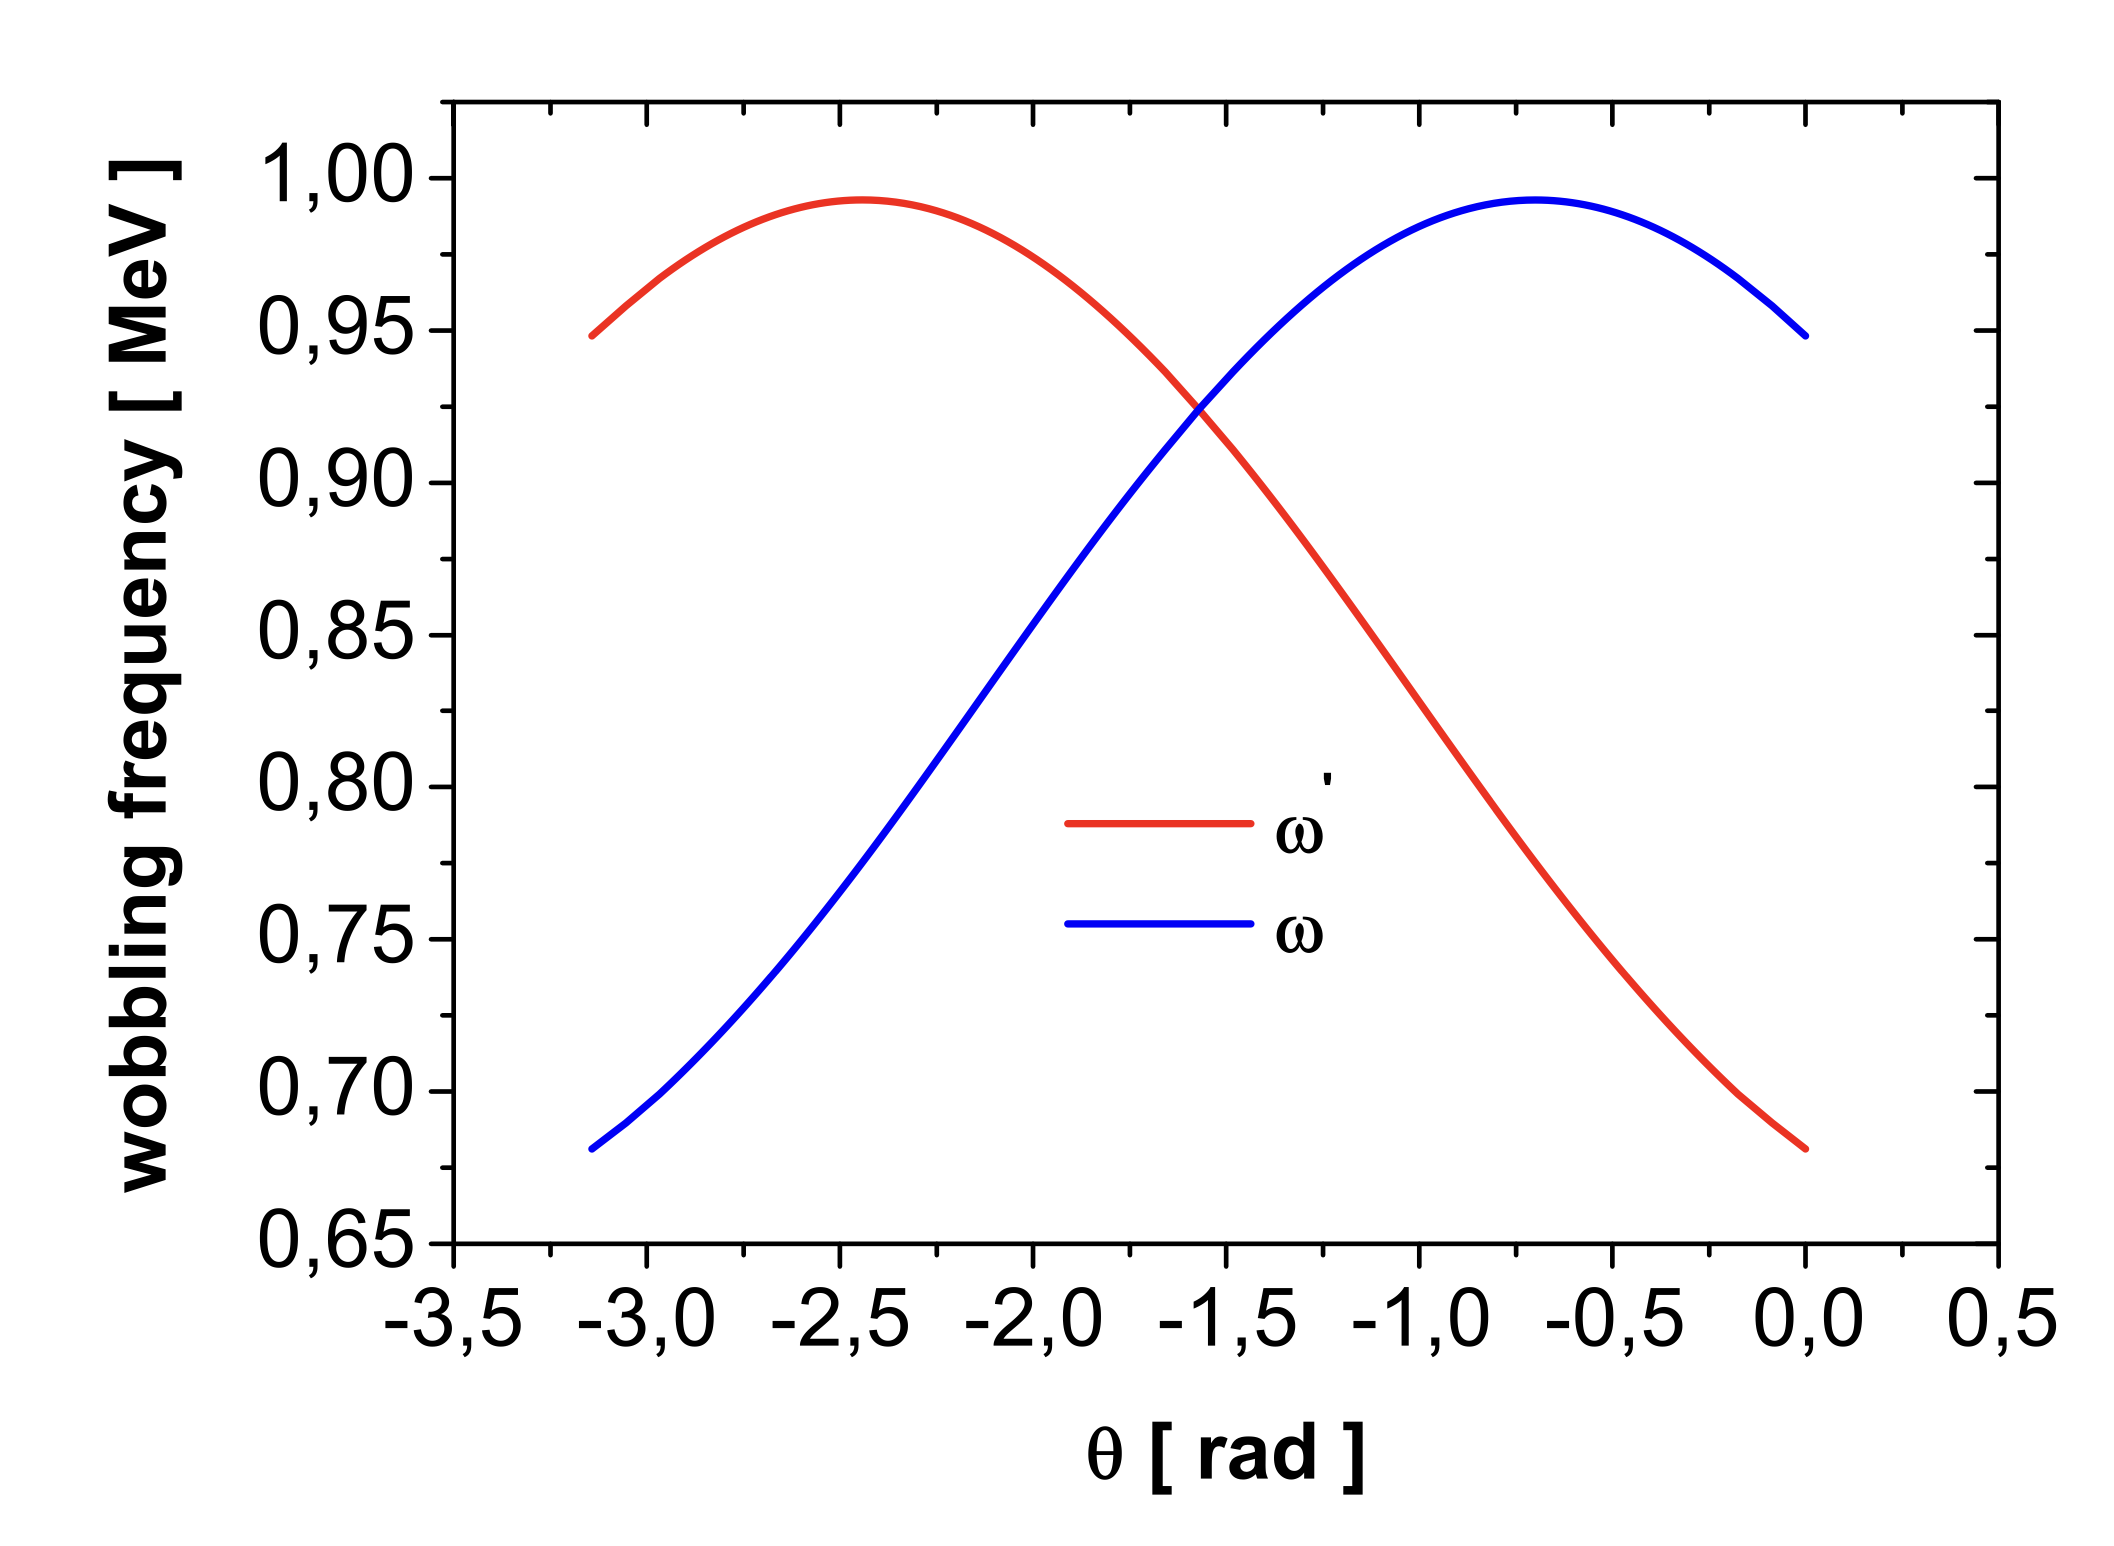
\includegraphics[scale=0.18]{figures/wobbling-frequencies.png}
  \caption{$j=13/2$, $I=55/2$.}
\end{figure}
\end{frame}

\section{Numerical application - energy spectrum}

\begin{frame}
  \frametitle{Numerical Results}
  \begin{itemize}
    \item Find the excitation energies for a nucleus using the obtained analytical results $E_n$.
    \item Applied the formalism on the wobbling spectrum of $^{135}$Pr.
    \item Experimental confirmation for three wobbling bands (Matta et al. 2015).
  \end{itemize}

  \begin{block}{Fitting procedure}
    \begin{itemize}
      \item Moments of inertia $\mathcal{I}_{1,2,3}$ are set as free parameters.
      \item Angle $\theta$ is also a free variable.
      \item $^{135}$Pr ($Z=59$, $N=76$) has $j=11/2$ (proton from the $h_{11/2}$ orbital).
      \item \textbf{Fitted MoI:} $\mathcal{I}_1:\mathcal{I}_2:\mathcal{I}_3=91:9:51\ [\hbar\text{MeV}^{-1}]$.
      \item \textbf{Fitted} $\theta$: $-119$ degrees ($-2.07694$ rad).
      \item $E_\text{rms}=0.170$ MeV.
    \end{itemize}
  \end{block}
\end{frame}

\begin{frame}
  \frametitle{Excitation Energies}
\begin{figure}
  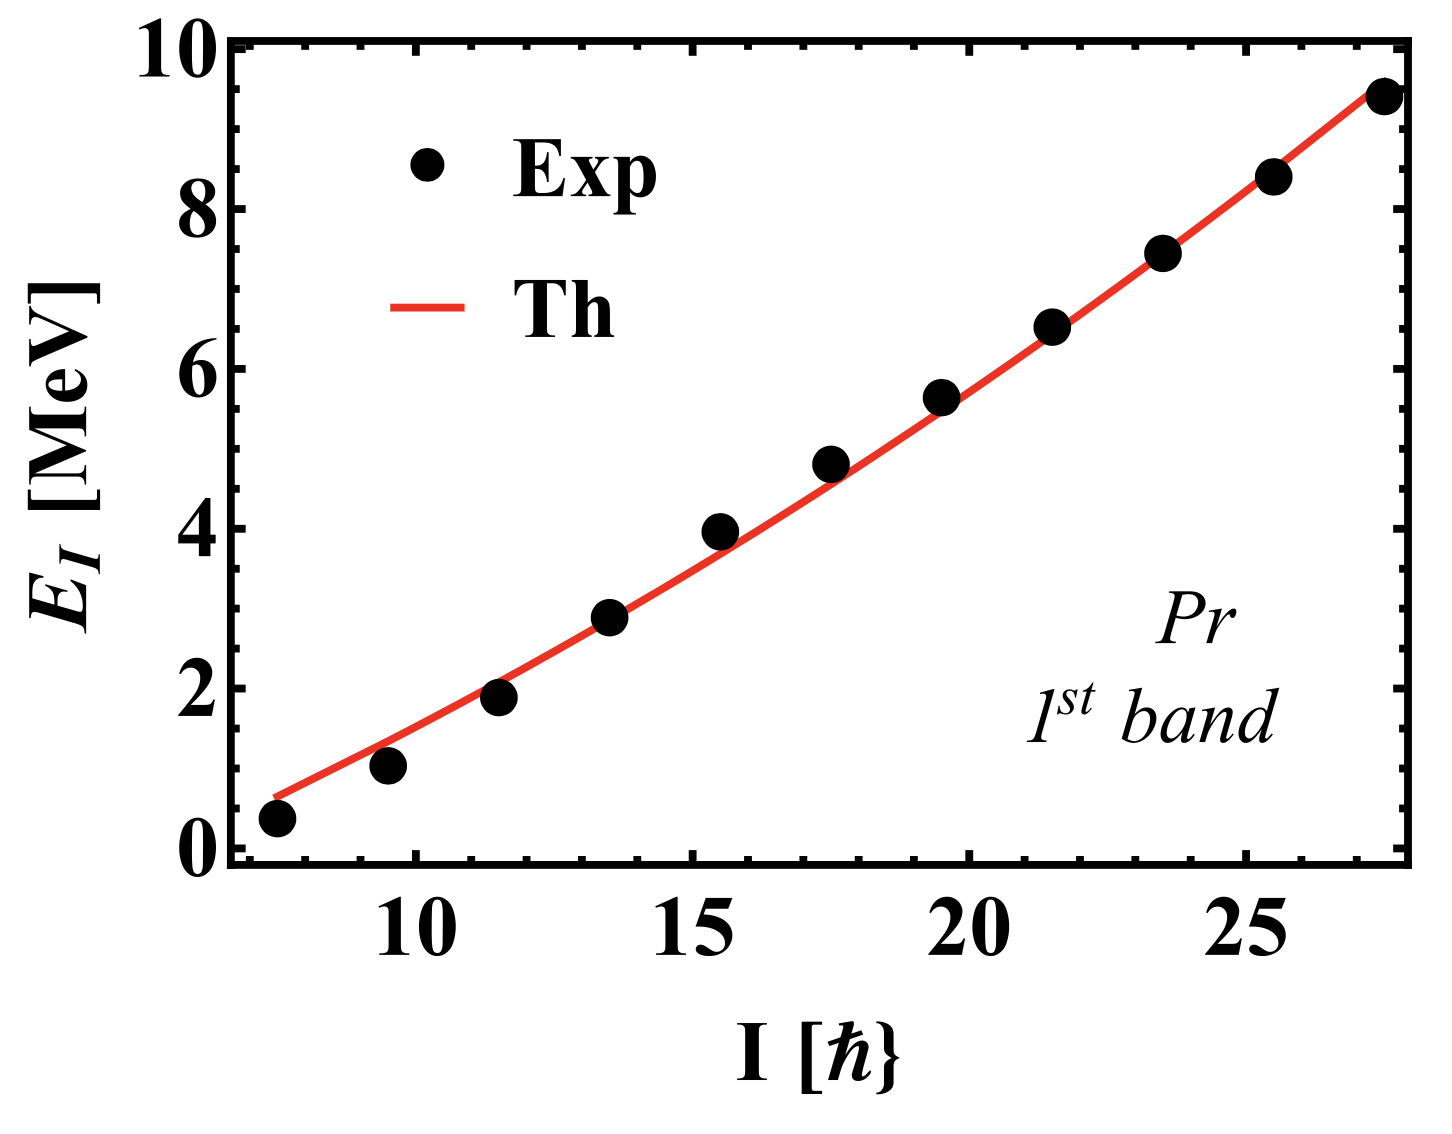
\includegraphics[scale=0.18]{figures/energy_1.png}
  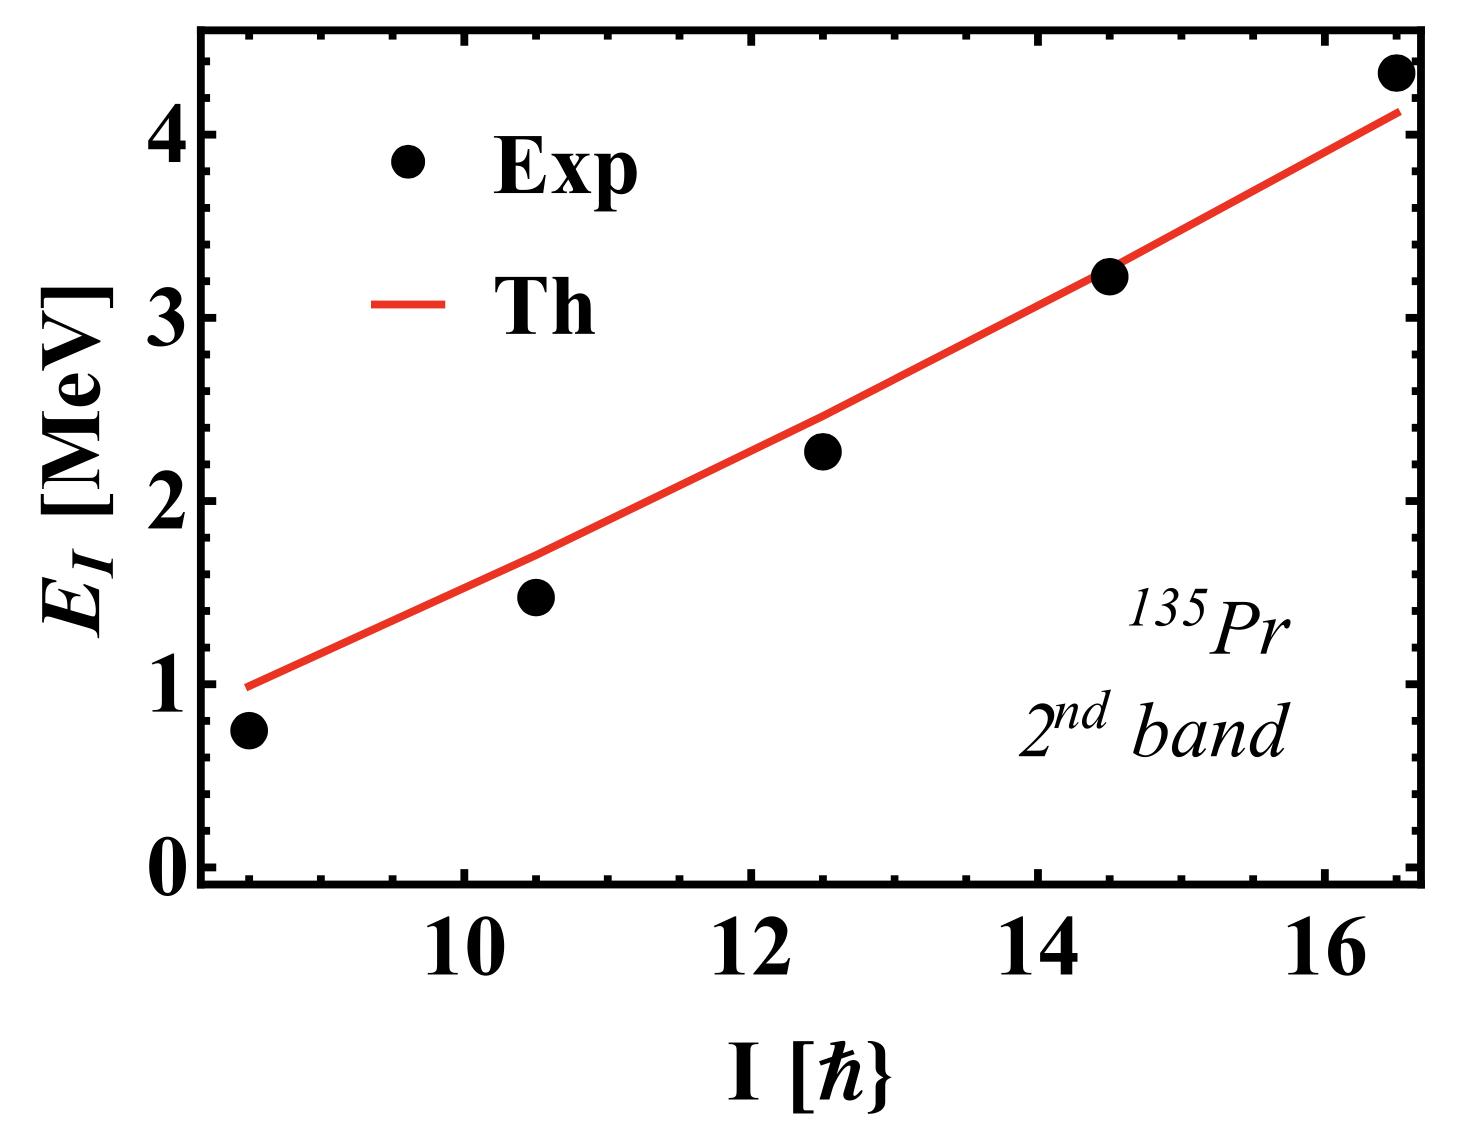
\includegraphics[scale=0.18]{figures/energy-2.png}
  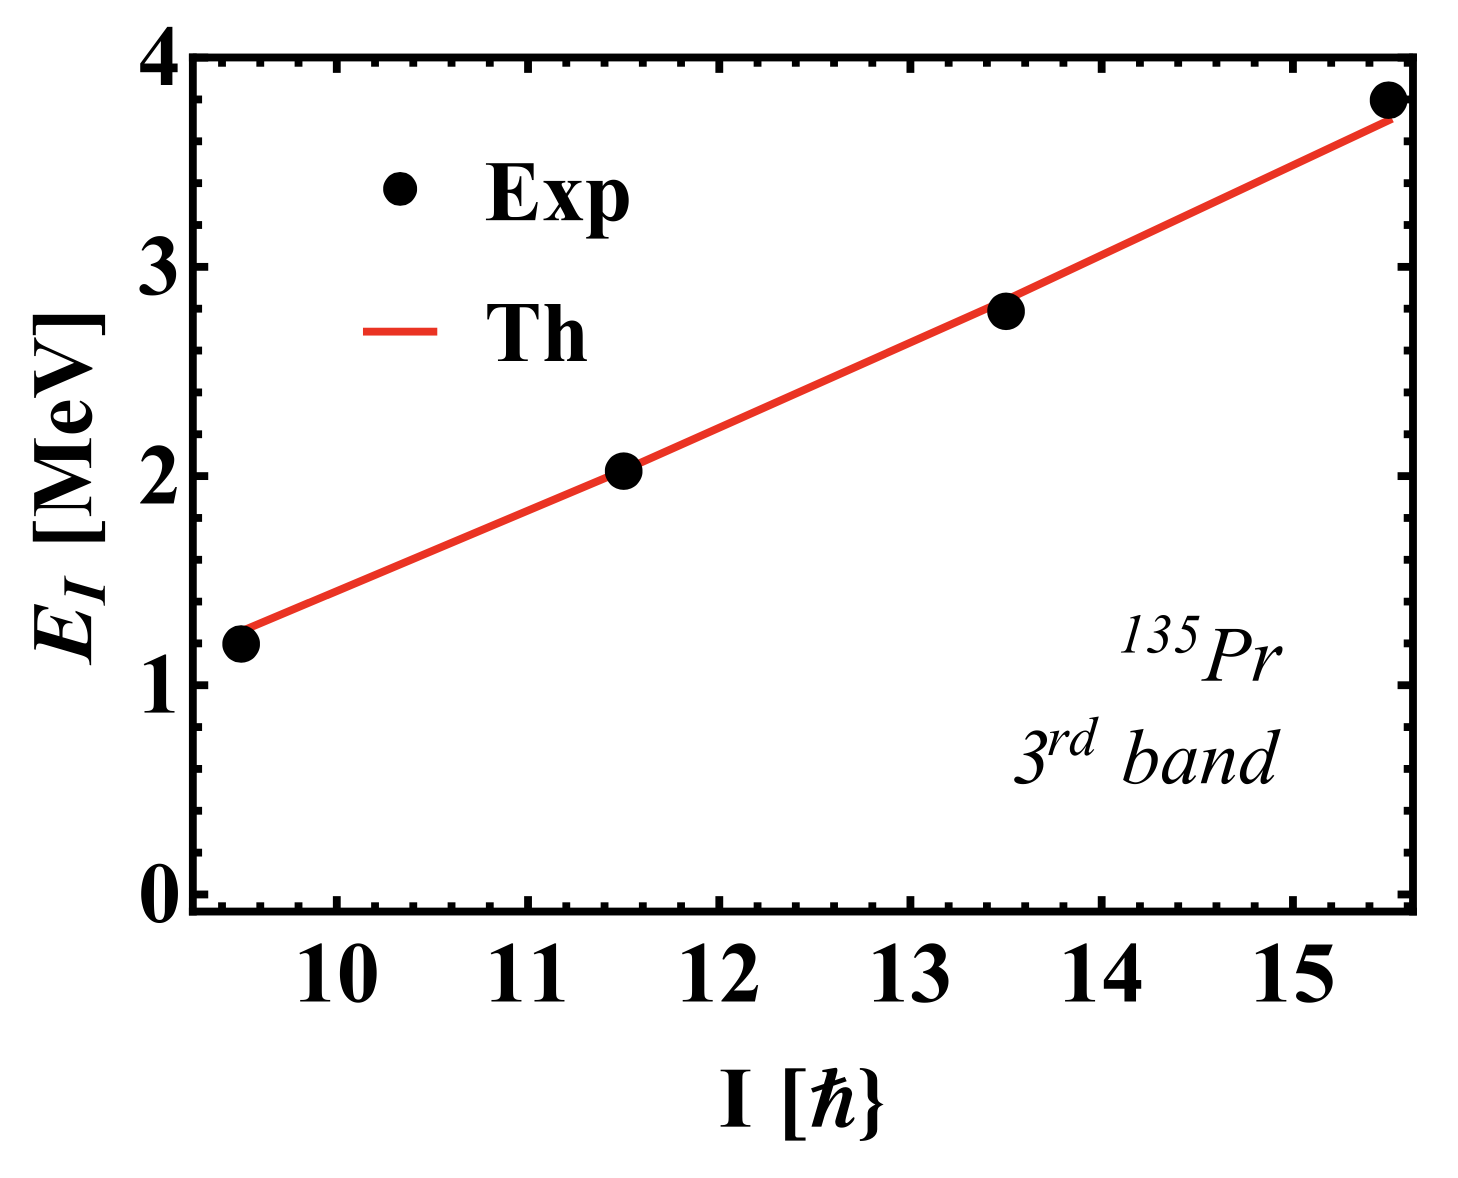
\includegraphics[scale=0.18]{figures/energy-3.png}
\end{figure}
\end{frame}

\begin{frame}
  \frametitle{Elliptic potential}
\begin{figure}
  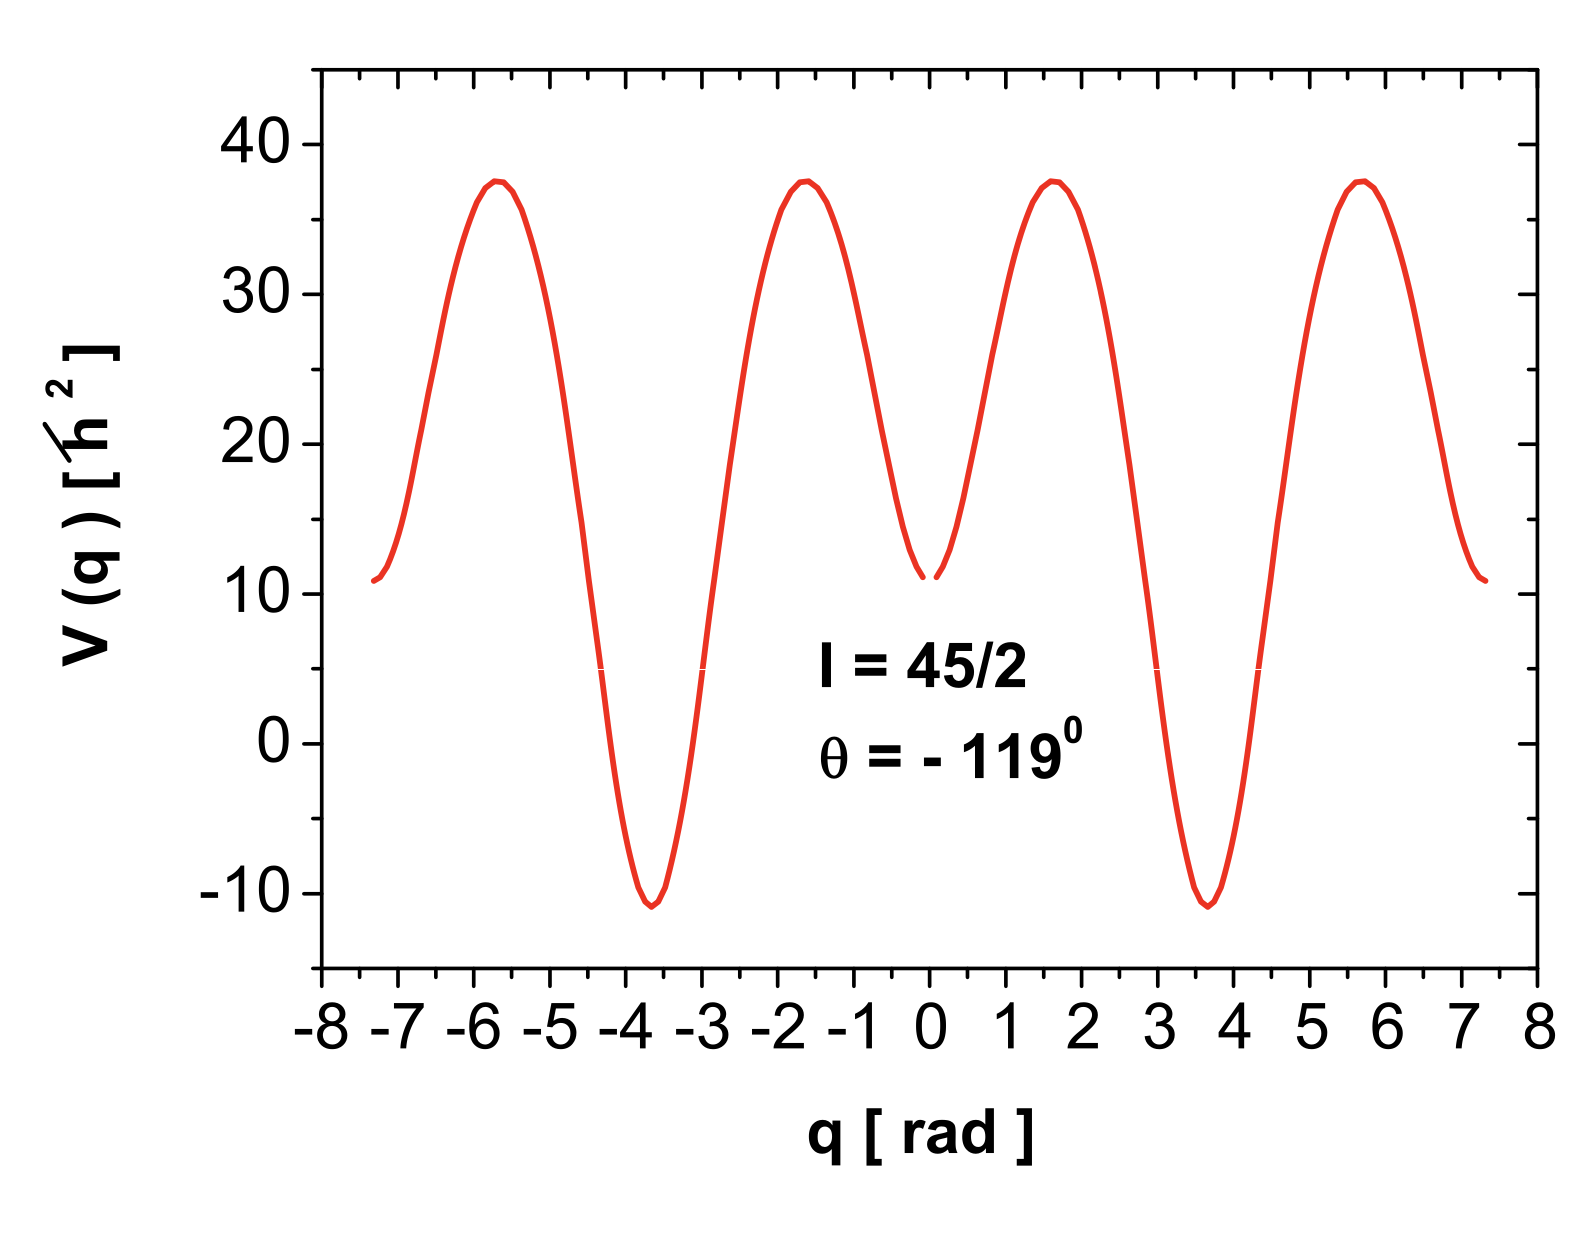
\includegraphics[scale=0.2]{figures/potential-pr-135.png}
  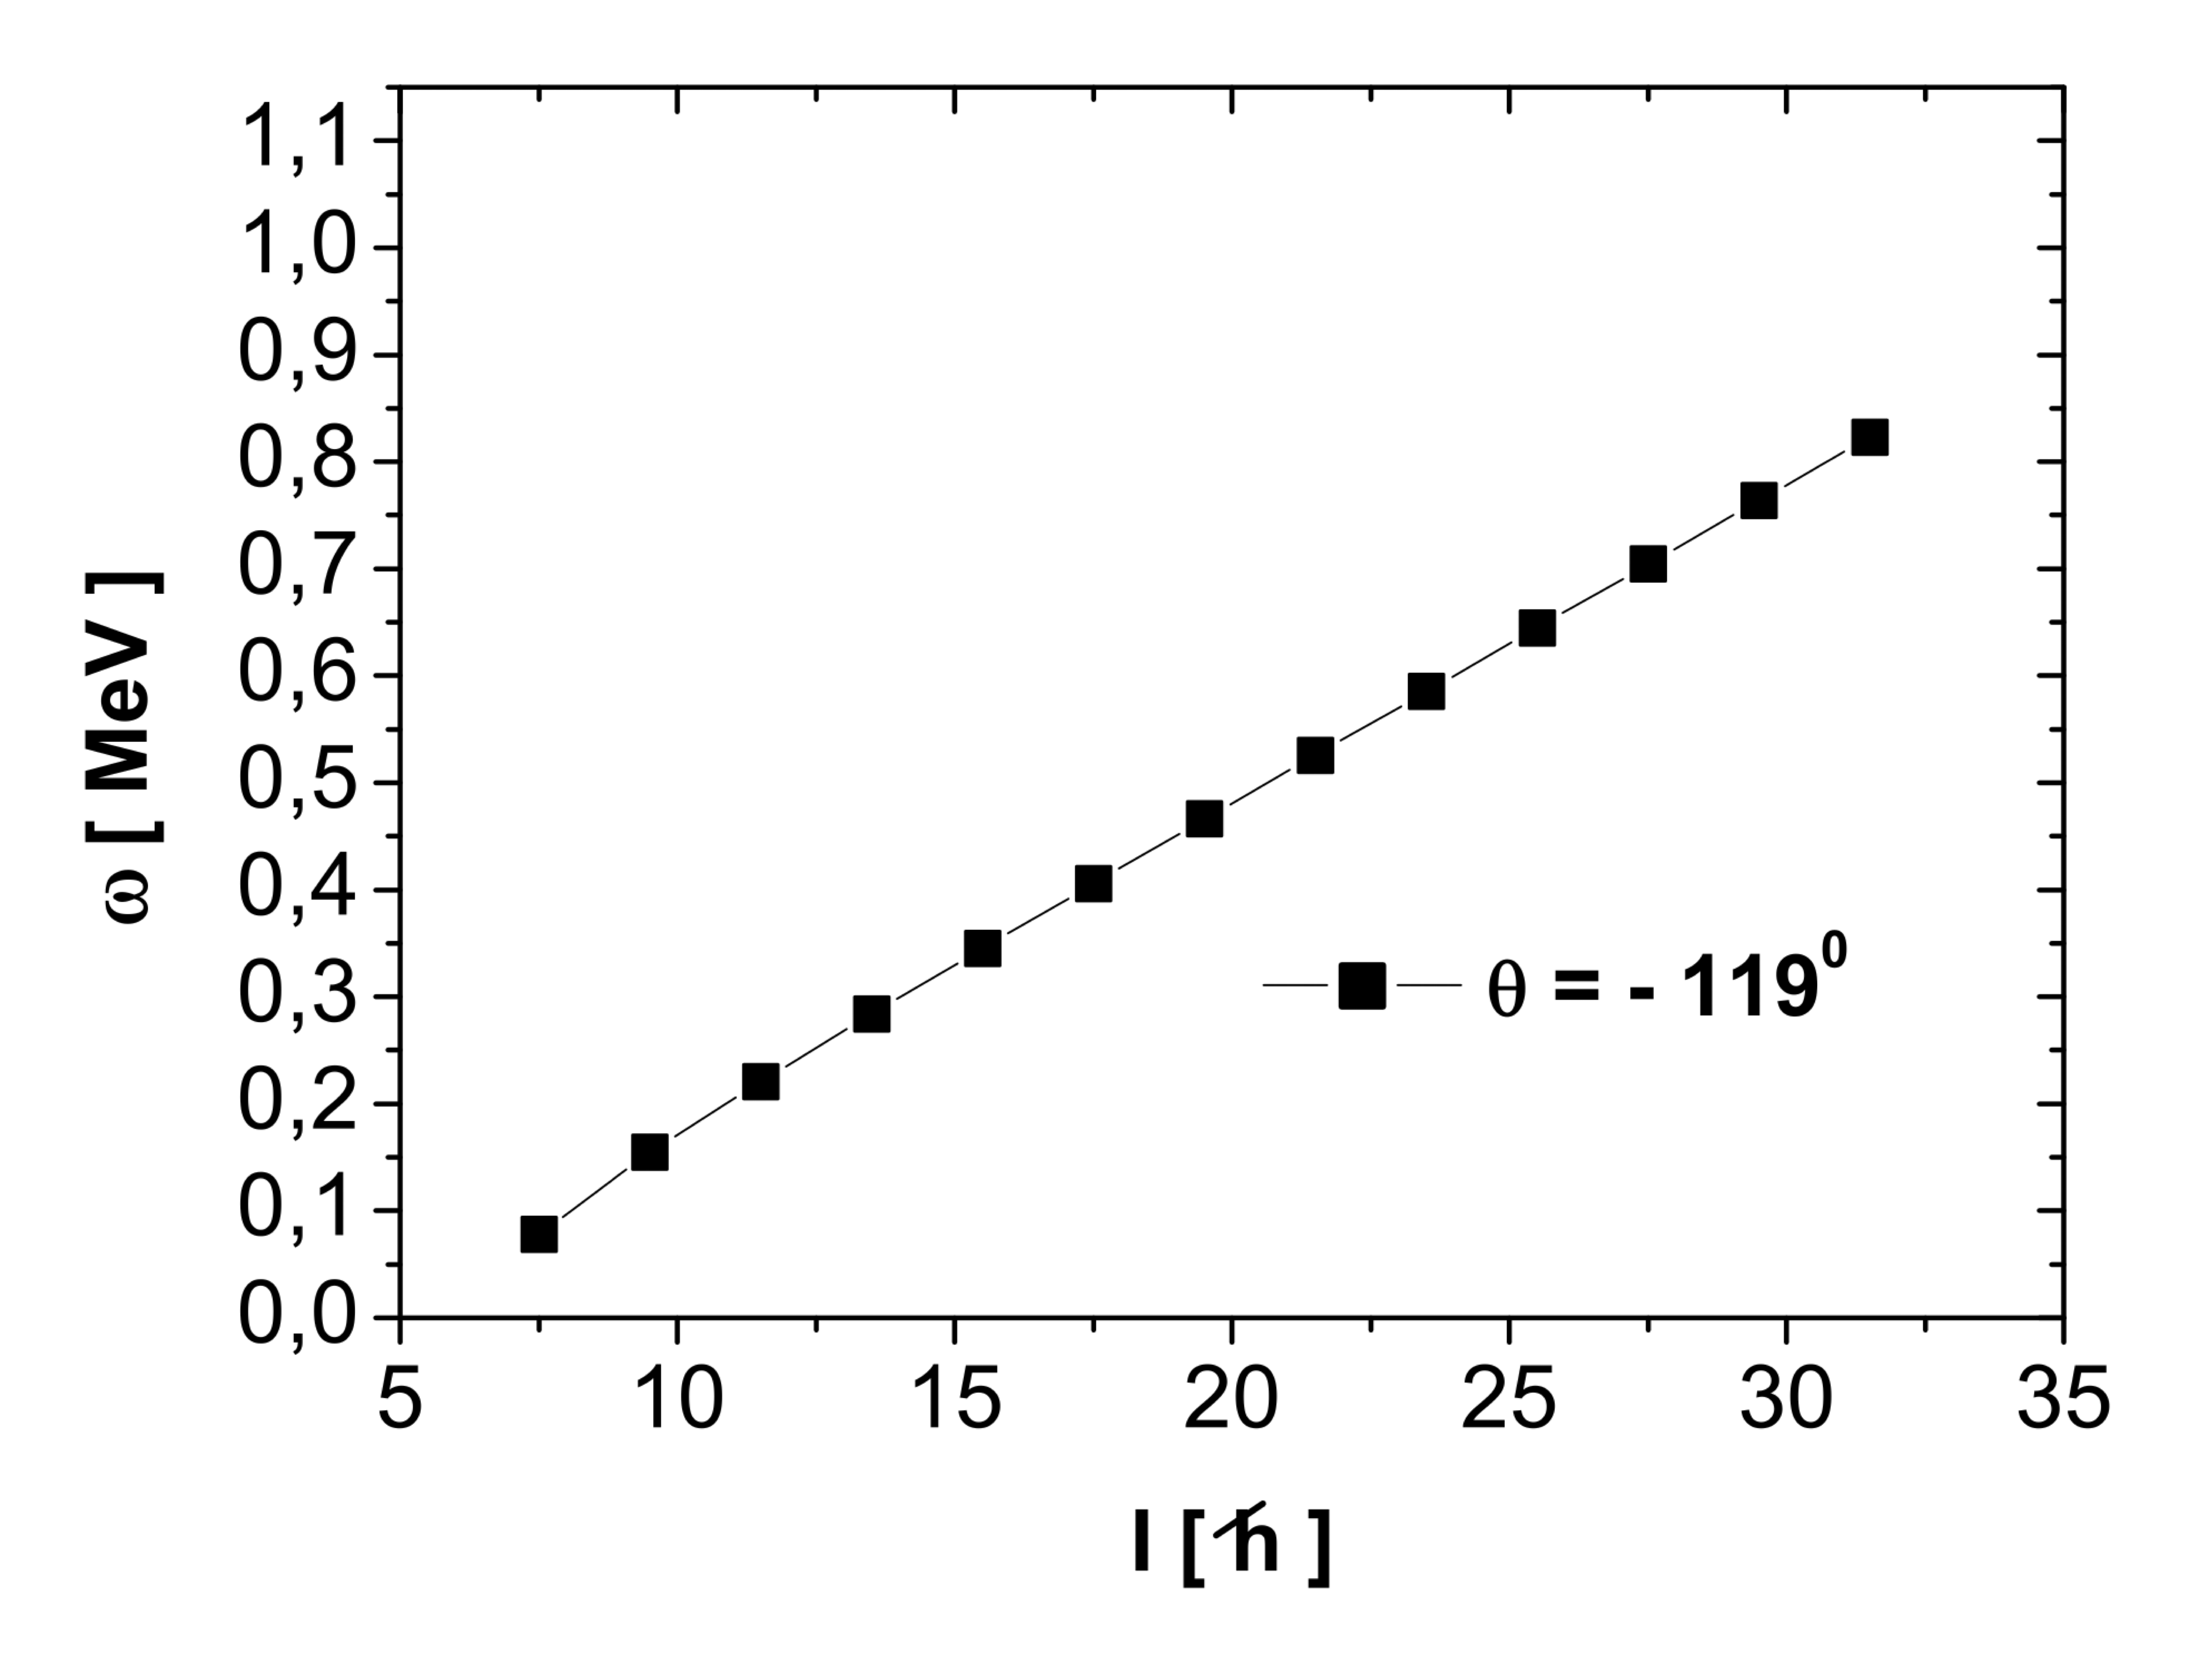
\includegraphics[scale=0.04]{figures/frequencies-pr-135.png}
\end{figure}
\begin{itemize}
  \item Contribution coming from the wobbling frequency is rather small.
  \item Potential exhibits local minima and deep minima.
  \item Stability of the wobbling motion is characterized by $q\sim3-4$ rad.
\end{itemize}
\end{frame}

\section{Conclusions}

\begin{frame}
  \frametitle{Conclusions}
  \begin{itemize}
    \item The Hamiltonian for an odd-mass nucleus $H_\text{rot}$ is described based on the coupling between \emph{triaxial even-even core} and an odd particle.
    \item $H_\text{rot}$ is split up in three terms: $H'$, $H_{sp}$, and a spin term.
    \item Treating $H'$ through the variables $q,d/dq$, one obtained a Schrodinger equation with separated kinetic and potential terms.
    \item The potential term $V(q)$ is expressed in terms of the Jacobi elliptic functions $s,c,d$.
    \item Bargmann mapping changes the a.m. components to boson operators.
    \item Expansion of $V(q)$ up to second order in $q$ is used to obtain $E_n$.
    \item Spectrum of $^{135}$Pr is described, reproducing the energies for the three wobbling bands.
  \end{itemize}
\end{frame}

\begin{frame}
  \frametitle{}
  \begin{center}
    {\Huge Thank you for your attention!}
  \end{center}
\end{frame}
\end{document}
